% !TEX Program = lualatex
% class
\documentclass[ngerman]{scrartcl}

% input preamble
\input{../../shared_preamble.tex}
\usepackage{framed}

% manual header
\ihead{Interferometrie}  % inner (left) head
\chead{\textsc{Wachmann} Elias (12004232)\\\textsc{Zach} Andreas (12004790)}  % center head
\ohead{10.03.2023}  % outer (right) head

\addbibresource{Interferometrie.bib}



\begin{document}

%%%%Title Page %%%%
\begin{titlepage}
    \centering
    \includegraphics[width=0.5\textwidth]{../../99_Misc/Logo_KF.pdf}\par\vspace{0.8cm}
    {\scshape\LARGE{Karl-Franzens-Universität Graz}\par}
    {\scshape\LARGE{Institut für Physik}\par}
    \vspace{1cm}
    {\scshape\Large{23S PHY.L02UB Fortgeschrittenenpraktikum 2}\par}
    678 Bachelorstudium Physik, UG2002/2021W\par
    \vspace{1.5cm}
    {\huge\bfseries II. Interferometrie\par}
    \vspace{2cm}
    \begin{table}[H]
        \centering
        \begin{tabular}{c c c}
            \Large Wachmann Elias &  & \Large Zach Andreas \\
            \Large 12004232       &  & \Large 12004790     \\
            \multicolumn{3}{c}{Gruppe 12}
        \end{tabular}
    \end{table}
    \vfill
    \Large Betreut von\par
    Thomas Georg \textsc{Boné}, BSc MSc

    \vfill

    % Bottom of the page
    {\large 10.03.2023\par}
\end{titlepage}
%%%%

\clearpage
\tableofcontents
\newpage

\section[Aufgabenstellung]{Aufgabenstellung \cite{ref:angabe}}
\label{sec:aufgabenstellung}

Der folgende Laborversuch besteht aus vier separaten Teilversuchen, welche sich abermals wie folgt in Unterversuche gliedern:

\begin{itemize}
    \item \textbf{Young'scher Doppelspalt}
          \begin{itemize}
              \item Bestimmen des Beugungsmusters von vier Doppelspalten mit unterschiedlichen Spaltbreiten und Spaltabständen
              \item Berechnung der Wellenlänge des Lasers
              \item Erklärung der Beugungsmuster durch Vergleich mit errechneten Mustern
              \item Bestimmung der Beugungsmuster eines Liniengitters und Vergleich mit errechneten Werten
              \item Bestimmung der Gitterkonstante
          \end{itemize}
    \item \textbf{Wellenfront-Analyse / Shearing Interferometer}
    \item \textbf{Polarisation}
          \begin{itemize}
              \item Verifizieren des Gesetzes von Malus
              \item Untersuchen des Einflusses des Durchlasswinkels eines weiteren Polarisators zwischen zwei gekreuzten Polarisatoren
          \end{itemize}
    \item \textbf{Michelson Interferometer}
          \begin{itemize}
              \item Justieren und generieren von konzentrischen Interferenzmustern
              \item Bestimmung der Wellenlänge des Lasers durch Weglängenänderung
              \item Untersuchung des absoluten Weglängenunterschieds in den beiden Interferometerarmen sowie Auflösung und Stabilität des Interferometers
              \item Untersuchung der Rolle der Polarisation auf die Interfenzfähigkeit des Laserlichts
          \end{itemize}
\end{itemize}


\section[Grundlagen]{Grundlagen \cite{ref:angabe}}
\label{sec:grundlagen}

\subsection{Young'scher Doppelspalt}
\label{sec:grundlagen_youngscher_doppelspalt}

Bescheint man mit einer Lichtquelle zwei eng beieinanderliegende Spalte mit dem Abstand $d$ und projiziert das Bild auf einen ansonsten undurchsichtigen Schirm, so wirkt der Spalt als kohärente Lichtquelle (Anmerkung: Dies ist evident für eine kohärente Lichtquelle, gilt für eine thermische Lichtquelle aber nur unter bestimmten Bedingungen, jenen der räumlichen Kohärenz). Die Wellen aus den Spalten überlagern sich in Abhängigkeit vom Beobachtungswinkel konstruktiv oder destruktiv, was auf einen Schirm projiziert eine Abfolge an Intensitätsmaxima und -minima ergibt. Unter der Bedingung, dass der Abstand zwischen Doppelspalt und Beobachtungsebene viel größer als der Spaltabstand $d$ ist, ergibt sich der optische Gangunterschied in die durch den Winkel $\phi$ definierte Richtung als
\begin{equation}
    \Delta = \frac{2 \pi d}{\lambda} \sin(\phi)
\end{equation}
mit $\lambda$ der Wellenlänge.
Mit der Näherung $\sin(\phi) \approx \nicefrac{x}{z}$ (erfüllt für große Abstände $z$ zwischen Doppelspalt und Schirm) ergibt sich ein Streifenmuster mit der Periode $x$ der Form
\begin{equation}
    I_{\text{Interferenz}}(x) = I_0 \left(1 + \cos(\frac{2 \pi x d}{\lambda z}) \right)
\end{equation}
Dafür wurde die endliche Breite des Spalts vernachlässigt bzw. ein unendlich schmaler Spalt angenommen. Tatsächlich überlagert sich dem Interferenzmuster das Beugungsmuster des Einzelspalts, das i.A. symmetrisch mit zu größeren Winkeln hin abnehmender Intensität ist. Ein einzelner rechteckiger Spalt der Breite $D$ führt zu einem Beugungsmuster der Form
\begin{equation}
    I_{\text{Beugung}}(x) = I_0 \cdot \frac{\sin^2(\frac{\pi D x}{\lambda z})}{\left(\frac{\pi D x}{\lambda z}\right)^2}
\end{equation}
Das Beugungsmuster des Doppelspalts ergibt sich multiplikativ als
\[I(x) = I_{\text{Interferenz}}(x) \cdot I_{\text{Beugung}}(x).\]%
%
%
\subsection{Shearing-Interferometer / Wellenfront-Analyse}
\label{sec:grundlagen_shearing_interferometer}

Das Erscheinungsbild von optischen Interferenzmustern ist sowohl durch die Natur der Lichtwelle als auch der optischen Grenzflächen bestimmt, man denke an die färbigen Interferenzen auf Seifenblasen. Entsprechend ist es möglich, aus der Beobachtung von Interferenzen an Grenzflächen bekannter Geometrie auf die Eigenschaften der Lichtwelle zu schließen.
%? Evtl. Bilder
Beim Shearing-Interferometer handelt es sich um ein simples Interferometer, mit dem bestimmt werden kann, ob ein Lichtstrahl kollimiert, konvergent oder divergent ist. Dazu trifft das Licht unter \SI{45}{\degree} auf eine Glasplatte (in Seitenansicht, siehe \autoref{fig:shearing_interferometer}a), welche keilförmig ausgeführt ist. Durch die Reflexion an der vorderen und hinteren Fläche der Glasplatte entstehen zwei reflektierte Strahlen (\autoref{fig:shearing_interferometer}a), in deren Überlappungsbereich Interferenz auftritt (\autoref{fig:shearing_interferometer}b). Durch die keilförmige Geometrie führt dies für einen kollimierten Strahl zu einem zur Einfallsebene des Lichts parallelen Streifenmuster (\autoref{fig:shearing_interferometer}b). Ein konvergierender bzw. divergierender Strahl führt dagegen nach \autoref{fig:shearing_interferometer}b zu einem gedrehten Streifenmuster. Aus dem lateralen Versatz der beiden reflektierten Strahlen $l$, dem Streifenabstand $s$ und dem (auf die Senkrechte bezogenen) Winkel der Interferenzstreifen $\Theta$ (siehe \autoref{fig:shearing_interferometer}b) lässt sich der Radius $r$ der Wellenfront mit
\[r = \frac{ls}{\lambda \cdot \sin(\Theta)}\]
berechnen.

\begin{figure}[H]
    \centering
    \begin{samepage}
        \includegraphics[width=0.8\linewidth]{fig/Angabe_Abb5.png}
        \caption[Shearing-Interferometer]{Shearing-Interferometer. (a) Schematischer Aufbau in Seitenansicht, (b) beobachtete
            Interferenzmuster (in Aufsicht) für kollimierte, konvergierende und divergierende Wellenfronten, im
            mittleren Bild sind die im Text besprochenen Bestimmungsgrößen eingezeichnet. \copyright{} Thorlabs, Quelle: \cite{ref:angabe}}
        \label{fig:shearing_interferometer}
    \end{samepage}
\end{figure}


\subsection{Polarisation}
\label{sec:grundlagen_polarisation}

Für den Fall linearer Polarisation gilt für die transmittierte Intensität durch einen Polarisator mit der Durchlassrichtung entlang der durch den Winkel Null definierten Richtung das Gesetz von Malus.
\begin{equation}
    I(\alpha) = I_0 \cos^2(\alpha)
\end{equation}
Die nicht transmittierte Intensität wird je nach Art des Polarisators absorbiert oder reflektiert. Die Polarisation ist entscheidend für die Interferenzfähigkeit von Licht, es gelten die vier Gesetze nach Fresnel und Arago.
%? Is diese Anmerkung nötig?
%? \textbf{(siehe dazu auch einen entsprechenden Versuch mit dem Michelson-Interferometer)}.
\begin{framed}
    \begin{itemize}
        \item In dieselbe Richtung linear polarisierte Lichtstrahlen interferieren (wie nicht polarisiertes Licht).
        \item Zueinander senkrecht linear polarisierte Lichtstrahlen interferieren nicht (mit den nachfolgend aufgelisteten zwei Einschränkungen).
        \item Zueinander senkrecht linear polarisierte Lichtstrahlen interferieren, wenn sie ursprünglich dieselbe Polarisationsebene besaßen und wieder in diese zurückgeführt werden.
        \item  Zueinander senkrecht linear polarisierte Lichtstrahlen interferieren nicht, wenn sie in dieselbe Polarisationsebene zurückgeführt werden, diese aber nicht ursprünglich besaßen.
    \end{itemize}
\end{framed}

\subsection{Michelson-Interferometer}
\label{sec:grundlagen_michelson_interferometer}

Der prinzipielle Strahlengang eines Michelson-Interferometers ist in \autoref{fig:michalson_interferometer} dargestellt. Ein Lichtstrahl aus einer (Laser-)Quelle (1) wird an einem Strahlteiler (2) aufgeteilt. Der Strahlteiler ist ein dünnes Glasplättchen mit einer teilreflektierenden Schicht auf einer Fläche. Die beiden resultierenden Lichtstrahlen werden an zwei Spiegeln reflektiert und am Strahlteiler wieder vereint. Die Lichtstrahlen im Detektorarm treffen auf den Schirm (4), wo sie sich in Abhängigkeit vom Unterschied der Weglängen $s_1$ und $s_2$ überlagern. Für ebene Wellen der Form
\begin{equation}
    E(x,t) = E_0 e^{\omega t - k x}
\end{equation}
ist die Lichtintensität am Beobachtungsschirm gegeben durch
\begin{equation}
    I = \nicefrac{1}{4} \cdot c \cdot \varepsilon_0 \cdot E_0^2 \cdot (1 + \cos(\Delta \varphi))
\end{equation}
wobei $\Delta \phi$ die Phasendifferenz bezeichnet, die mit dem Unterschied der Weglängen\linebreak
$\Delta s = \left| s_1 - s_2 \right|$ nach $\Delta \varphi = (\nicefrac{2 \pi}{\lambda})\Delta s$ zusammenhängt.

\begin{figure}[H]
    \centering
    \begin{samepage}
        \includegraphics[width=0.6\linewidth]{fig/Angabe_Abb8.png}
        \caption[Michelson-Interferometer]{Michelson-Interferometer. Strahlengang im Michelson-Interferometer. Ein Laserstrahl aus der Quelle (1) wird am Strahlteiler (2) aufgeteilt, die beiden Teilstrahlen durchlaufen die beiden Interferometerarme der Länge s1 und s2. Nach ihrer Reflexion an den Spiegeln (3,4) werden die Teilstrahlen am Strahlteiler wieder überlagert und interferieren am Beobachtungsschirm (4). \copyright{} Thorlabs, Quelle: \cite{ref:angabe}}
        \label{fig:michalson_interferometer}
    \end{samepage}
\end{figure}

Es stellt sich die Frage, wo bei destruktiver Interferenz im Detektorarm die Energie der Lichtwellen bleibt. Tatsächlich hat das Interferometer ja zwei \enquote{Ausgänge}, wobei einer eben zum Beobachtungs-schirm, der zweite zurück zum Laser führt. Tatsächlich beobachtet man in zweiterem konstruktive Interferenz, wenn am Schirm destruktive Interferenz (also keine Lichtintensität) zu beobachten ist.

Das am Schirm beobachtete Interferenzmuster reagiert empfindlich auf kleine Änderungen in der Richtung des einfallenden Laserstrahls und in der Ausrichtung der Spiegel. Gleichzeitig sind diese Änderungen durch den nur wenige mm durchmessenden Strahl schwer zu beobachten. Deshalb wird der Strahl durch eine Linse aufgeweitet, was zwischen Laser und Strahlteiler oder zwischen Strahlteiler und Schirm geschehen kann. Ersteres führt zu einem konzentrischen Interferenzmuster, zweiteres zu parallelen Interferenzstreifen. Wie in \autoref{fig:interferenzmuster_michelson_interferometer}a skizziert, können divergierende Strahlen auf (bei Vorliegen eines Weglängenunterschieds $\Delta s$ zwischen den beiden Interferometerarmen) auf zwei virtuelle Lichtquellen A und B zurückgeführt werden, wodurch sich das Auftreten eines konzentrischen Interferenzmusters erklärt. Gleichzeitig kann dieses genutzt werden, um die Interferometerarme auf die gleiche Länge einzustellen (im Prinzip auf einen Bruchteil der Wellenlänge), da sich dabei nach \autoref{fig:interferenzmuster_michelson_interferometer}b die Größe des zentralen Interferenzspots maximiert. Alternativ könnte dazu eine breitbandige Lichtquelle mit geringer Kohärenzlänge verwendet werde, wobei die Kohärenzlänge durch die Verwendung von Bandpassfiltern erhöht werden kann.

\begin{figure}[H]
    \centering
    \begin{samepage}
        \includegraphics[width=\linewidth]{fig/Angabe_Abb9.png}
        \caption[Interferenzmuster Michelson-Interferometer]{Zum kreisförmigen Interferenzmuster beim Michelson-Interferometer. (a) Skizze zur Erklärung seiner Entstehung, (b) Skizze zur Erklärung der Größe des zentralen Maximums (oder Minimums). \copyright{} Thorlabs, Quelle: \cite{ref:angabe}}
        \label{fig:interferenzmuster_michelson_interferometer}
    \end{samepage}
\end{figure}

\clearpage

\section{Geräteliste}
\label{sec:geraeteliste}

Für den praktischen Aufbau und die Messungen der geforderten Größen wurden die in \autoref{tab:geraeteliste} aufgelisteten Geräte und Hilfsmittel verwendet.

\begin{table}[H]
    \centering
    \begin{samepage}
        \caption[Geräteliste]{Verwendete Geräte und wichtige Materialien}
        \label{tab:geraeteliste}
        \begin{tblrx}{cells={font=\footnotesize}}
            Gerät & Hersteller & Modell & Messsbereich / Unsicherheit & Inventar-Nr. \\
            Laser & Thorlabs & CPS532 &$\lambda = 532$&22442-S01\\
            diverse Spiegel & Thorlabs & KM100 &- &- \\
            Graufilter & Thorlabs & NX1N/M &- &- \\
            Doppelspalte & Phywe & 0852300 &- &- \\
            Gitter & Phywe & 0852400 &- &- \\
            Optischer Tisch& - & - &- &- \\
            diverse Halterungen & Thorlabs & - &- &- \\
            Sammellinse & Thorlabs & FMP1/M &f = $40$ mm &- \\
            Zerstreuungslinse & Thorlabs & FMP1/M &f = $-16$ mm &- \\
            Shearing-Interferometer & Thorlabs & nicht vorhanden &- &- \\
            Lichtintensitätsmesser & Sauter & SO 200k & $\Delta I = (\pm \SI{3}{\percent}\text{rdg} \pm \SI{0.5}{\percent}\text{fs}) \cdot I$ &51152203 \\
            Polarisationsfolie & Nitto denko & - &- &- \\
            Maßband& Schuller Eh klar& Power Tape \SI{3}{m}& Klasse II &- \\
            Michelson Interferometer & - & - &- &- \\
            Rohr & - & - &- &- \\
            diverse Abbildungsschirme & Wand, Papier, Tür, etc. & - &- &- \\
            Mobiltelefon & OnePlus & $8$-Pro &- &- \\
        \end{tblrx}
    \end{samepage}
\end{table}

Die verwendeten Doppelspalte haben die Abmessungen wie in \autoref{tab:doppelspalt_abmessungen} vermerkt.

\begin{table}[H]
    \centering
    \begin{samepage}
        \caption[Doppelspaltmaße]{Verwendete Doppelspalte mit der jeweiligen Nummer $i$, der Spaltbreite $D$ in \unit{\milli\meter} und dem Spaltabstand $d$ in \unit{\milli\meter}. Quelle: \cite{ref:angabe}}
        \label{tab:doppelspalt_abmessungen}
        \begin{tblr}{colspec={Q S[table-format=1.1]S[table-format=1.2]}, row{1}={guard}}
            $i$ / 1 & $D$ / \si{\milli\meter} & $d$ / \si{\milli\meter} \\
            1       & 0.2                     & 0.25                    \\
            2       & 0.1                     & 0.25                    \\
            3       & 0.1                     & 0.50                    \\
            4       & 0.1                     & 1.00                    \\
        \end{tblr}
    \end{samepage}
\end{table}

\paragraph{Anmerkung zu den Unsicherheiten:} Zur Unsicherheitsangabe werden die jeweiligen Unsicherheitsmaße der Geräte, welche aus den Datenblättern (sofern vorhanden) entnommen werden, verwendet. Für die analogen Messgeräte wird eine kombinierte Ablese- und Messunsicherheit von $\pm\SI{1}{Skalenstrich}$ verwendet.

Alle Teilversuche wurden bei einer Umgebungstemperatur von \SI{24(1)}{\celsius} einem Luftdruck von \SI{1000(10)}{\hecto\pascal} und einer relativen Luftfeuchtigkeit von \SI{33(1)}{\percent} durchgeführt.



\section{Versuchsaufbau}
\label{sec:aufbau}

\subsection{Young'scher Doppelspalt}
\label{sec:aufbau_doppelspalte}

Für den Aufbau zum Versuch \textit{Young'scher Doppelspalt} wird der Laser mittels zwei Spiegel auf das Plättchen mit den vier verschiedenen (siehe \autoref{tab:doppelspalt_abmessungen}) Doppelspalten gelenkt. Der Abstand vom Doppelspalt wird mit \SI{2520(5)}{\milli\meter} bestimmt -- wobei hier noch zur vom Maßband gegebenen Unsicherheit von \SI{1.1}{\milli\meter} eine weitere Unsicherheit durch das Messen in der Luft hinzukommt. Der Aufbau in \autoref{fig:aufbau_doppelspalt} zeigt den optischen Tisch, der Schirm ist rechts im oben angeführten Abstand an der Wand befestigt.
\begin{figure}[H]
    \centering
    \begin{samepage}
        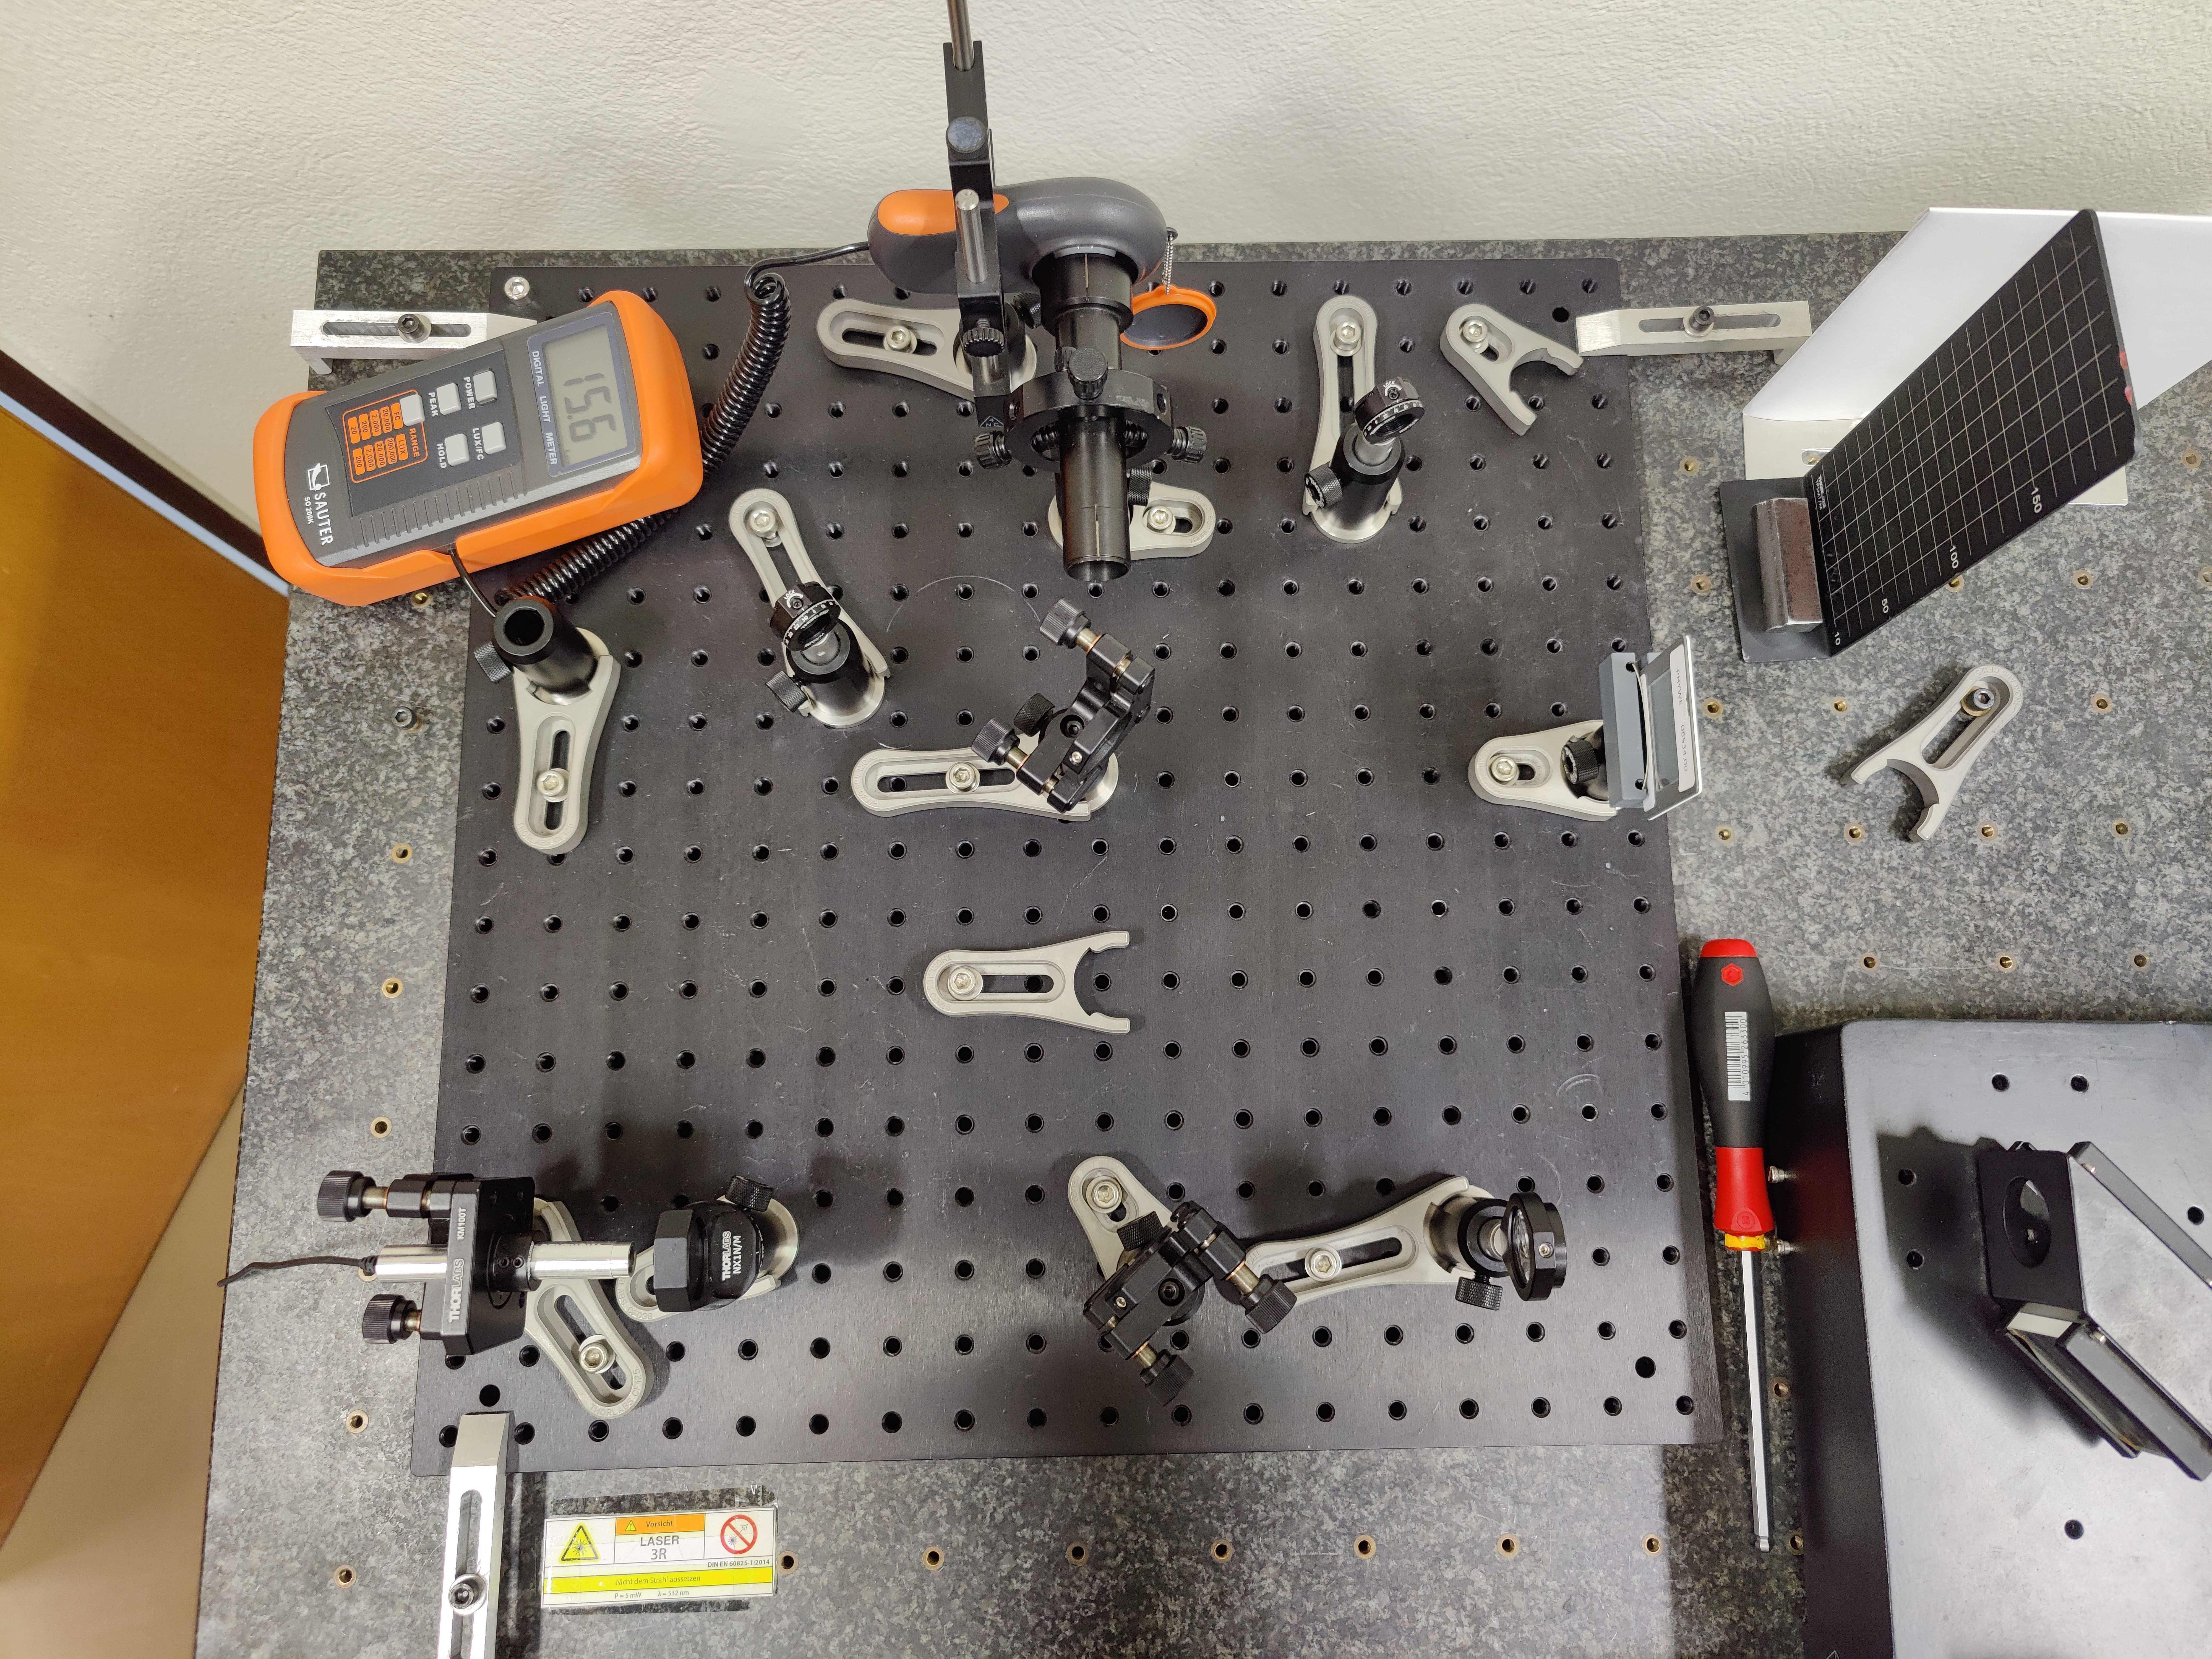
\includegraphics[width=0.7\linewidth]{fig/aufbau_doppelspalt.jpg}
        \caption{Aufbau Young'scher Doppelspalt}
        \label{fig:aufbau_doppelspalt}
    \end{samepage}
\end{figure}


\subsection{Shearing-Interferometer}
\label{sec:aufbau_shearing}

Der Aufbau des Shearing-Interferometers ist in \autoref{fig:aufbau_shearing} gegeben. Dabei wird der untere Spiegel aus dem vorhergehenden Versuch wiederverwendet und der Laserstrahl auf die Frontalebene gelenkt, welche um \SI{45}{\degree} zur Tischebene geneigt ist.
%
\begin{figure}[H]
    \centering
    \begin{samepage}
        \includegraphics[width=0.9\linewidth]{fig/shearing.jpg}
        \caption[Aufbau Shearing Interferometer]{Aufbau Shearing Interferometer. Quelle: \cite{ref:angabe}}
        \label{fig:aufbau_shearing}
    \end{samepage}
\end{figure}
%
\paragraph{Anmerkung zum Versuch:} Da sich das Shearing Interferometer leider zum Zeitpunkt der Übung in Reparatur befand, wird der Versuch im folgenden hyptotethisch abgehandelt.


\subsection{Polarisation}
\label{sec:aufbau_polarisation}

Anstelle des Shearing Interferometers werden jetzt zwei Polarisationsfilter in den Pfad des Lasers eingebracht. Nach dem zweitem Filter trifft der Laser auf einen Lichtintensitätsmesser, welcher wie in \autoref{fig:aufbau_polarisation} ersichtlich, durch ein Rohr von sonstigen Lichteinflüssen abgeschirmt wird.
%
\begin{figure}[H]
    \centering
    \begin{samepage}
        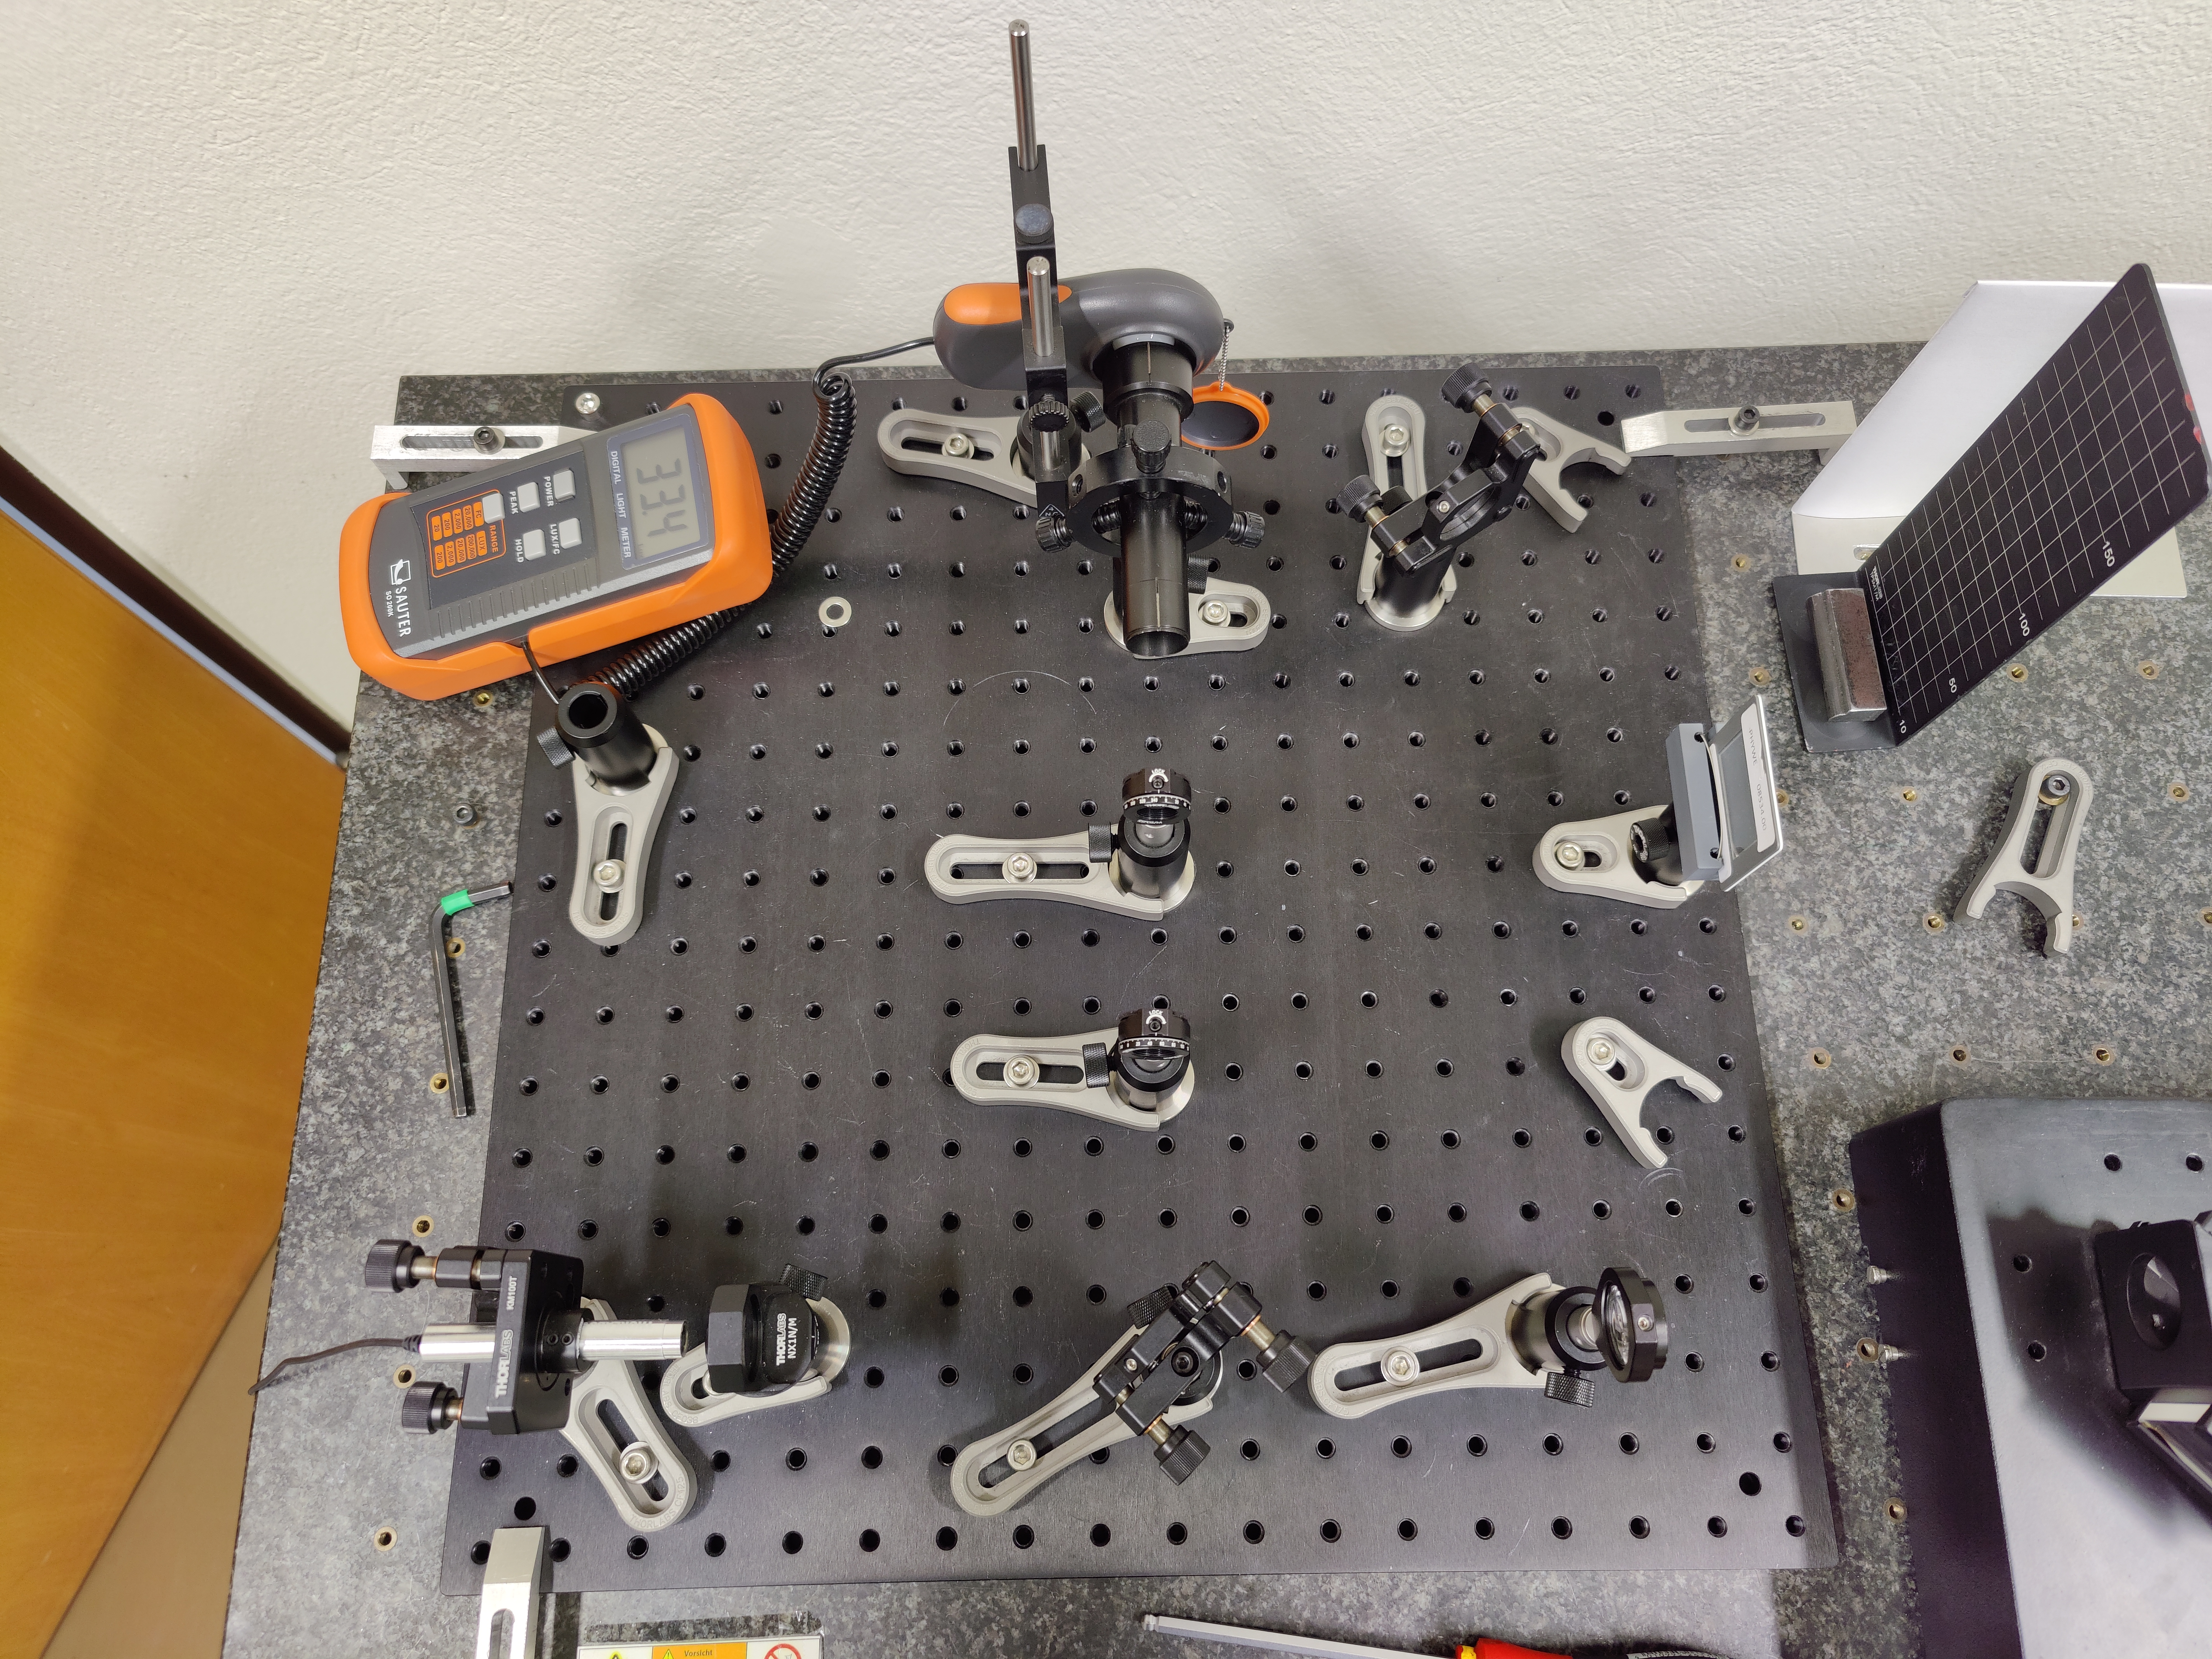
\includegraphics[width=0.7\linewidth]{fig/Aufbau_polarisation.jpg}
        \caption{Aufbau Polarisation}
        \label{fig:aufbau_polarisation}
    \end{samepage}
\end{figure}


\subsection{Michelson-Interferometer}
\label{sec:aufbau_michelson}

Nun wird auch der letzte verbleibende Spiegel aus dem Strahlengang des Lasers gegeben und der Laserstrahl trifft so direkt auf das in \autoref{fig:aufbau_michelson} rechts gezeigte Michelson-Interferometer. Wie gut in der Abbildung ersichtlich ist, wird der Strahl im Michelson-Interferometer in die beiden Arme aufgeteilt. Nach letztlicher Zusammenführung der beiden Strahlen trifft der resultierende Strahl auf den Schirm.
Zur Untersuchung verschiedener Effekte wird je eine Sammel- bzw. Zerstreuungslinse in den Strahlengang zwischen Laser und Michelson-Interfereometer eingebracht.
%
\begin{figure}[H]
    \centering
    \begin{samepage}
        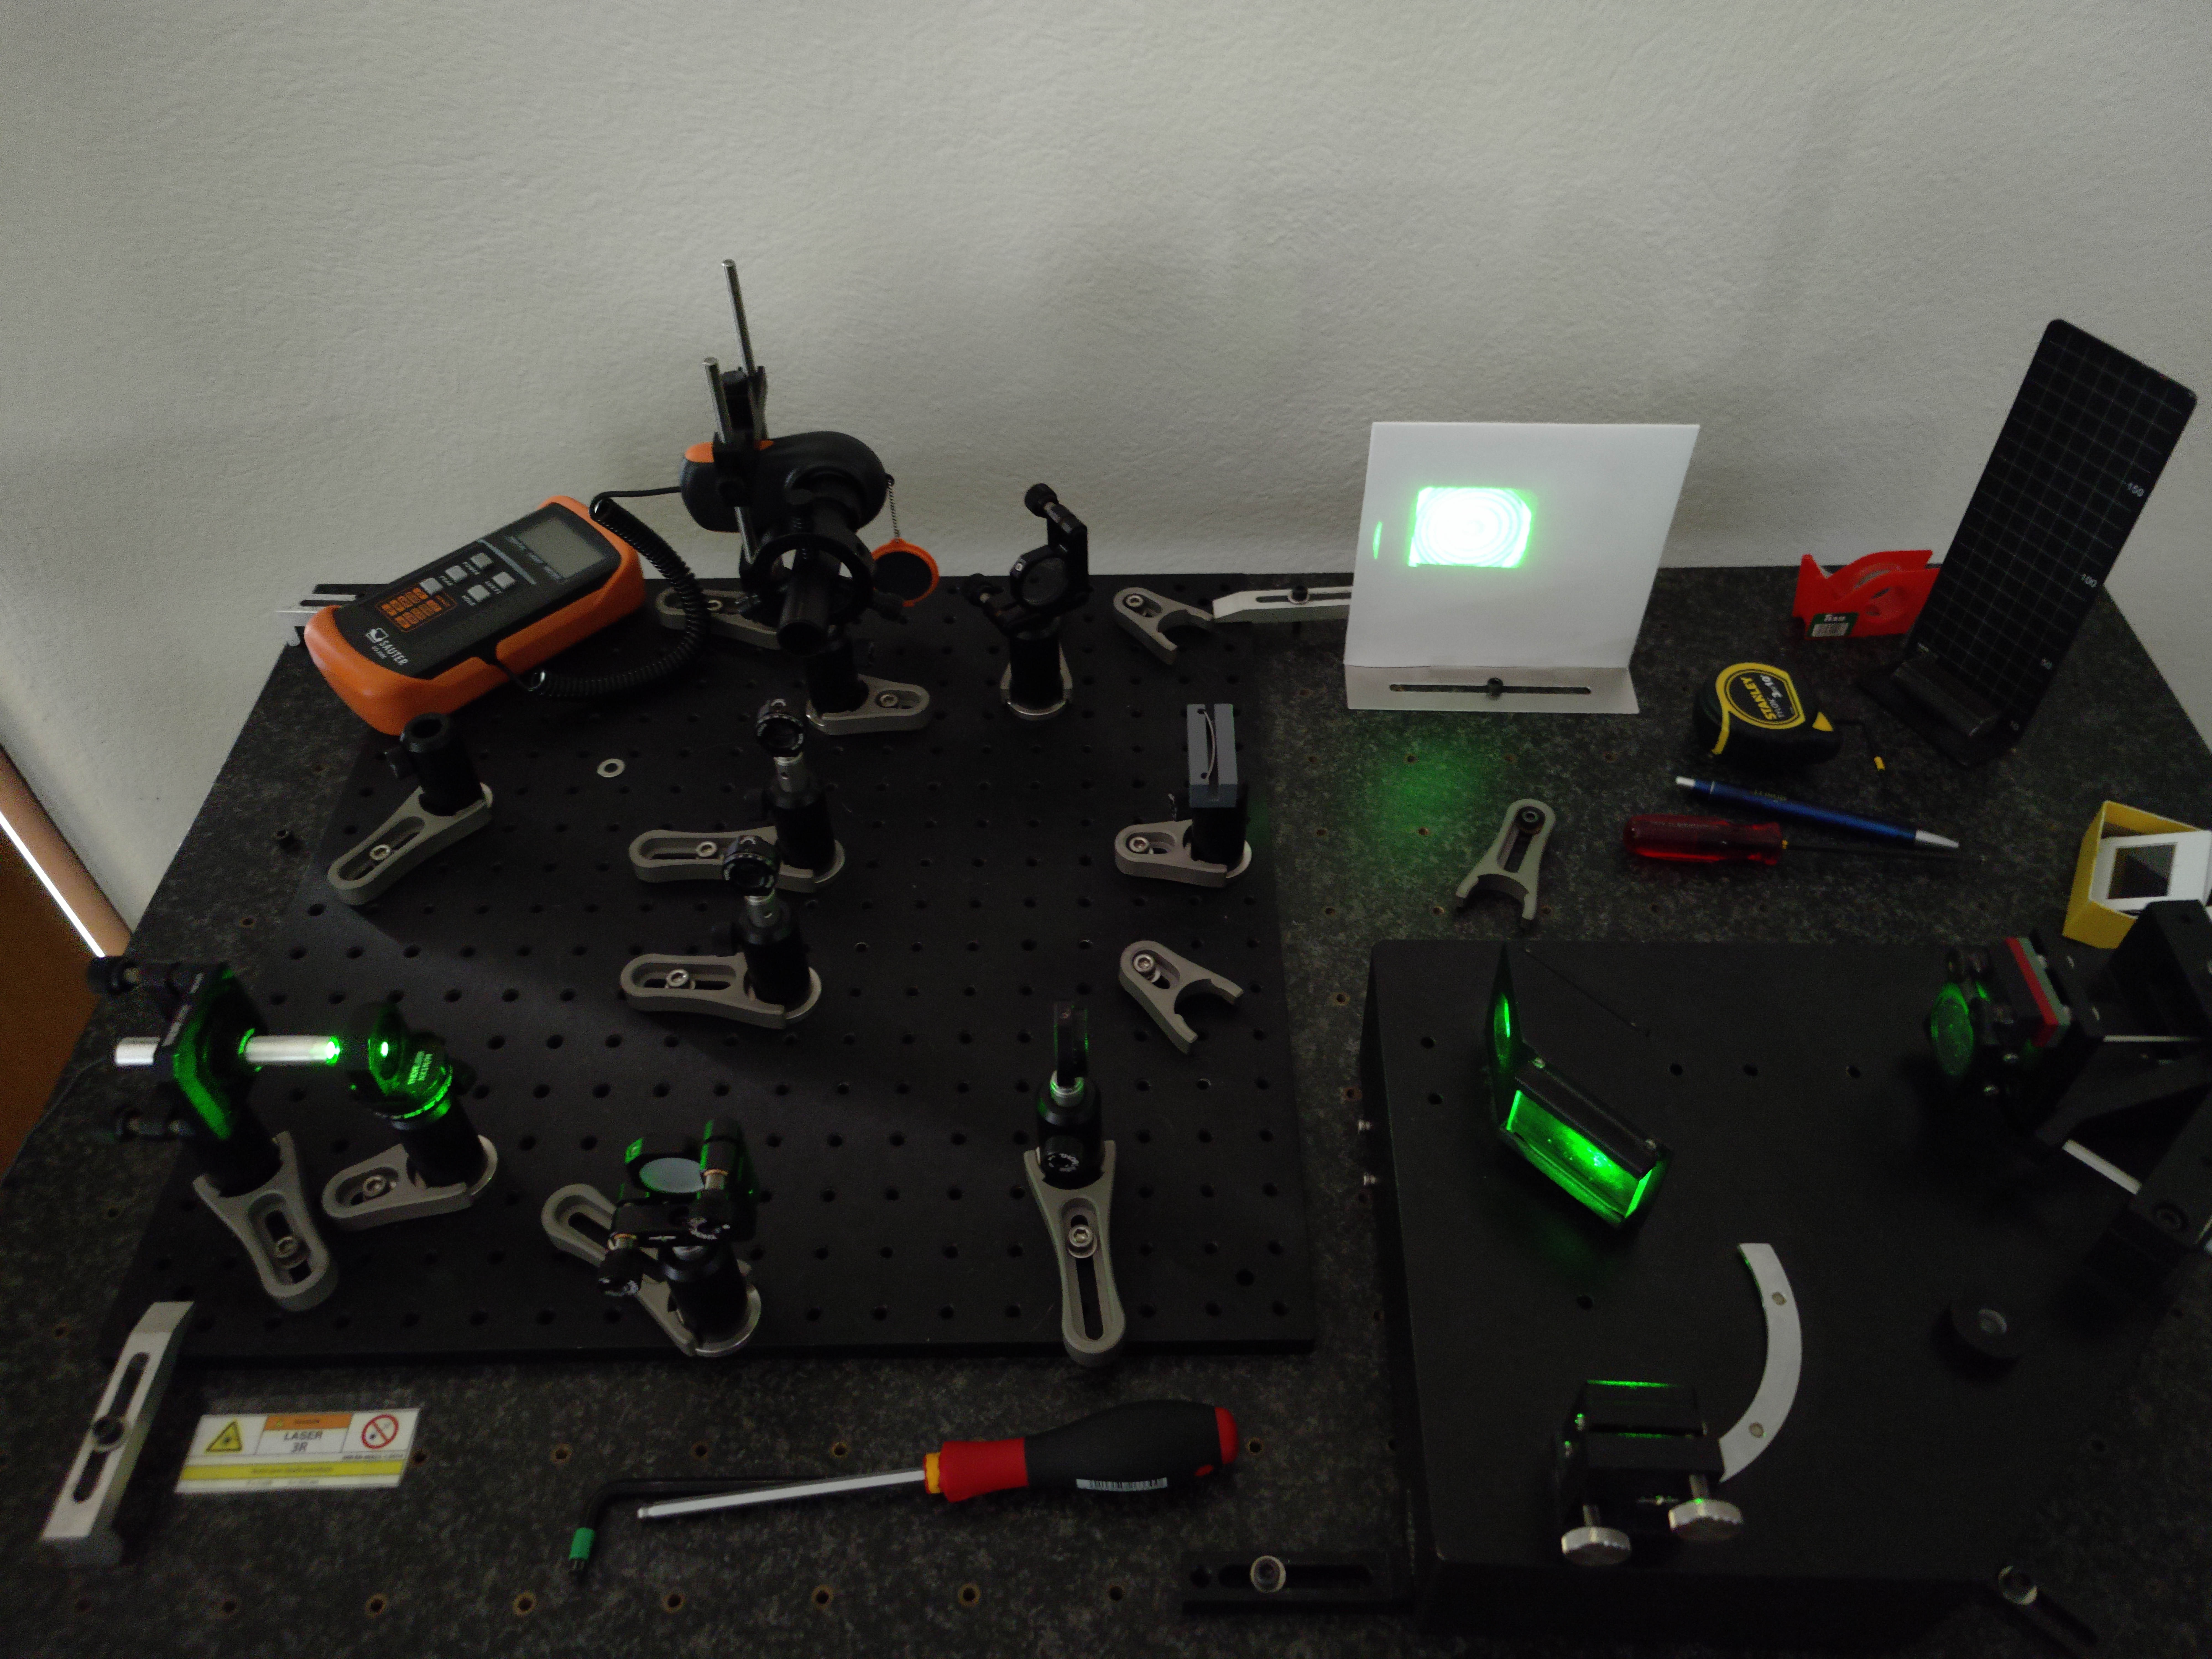
\includegraphics[width=0.7\linewidth]{fig/aufbau_michelson.jpg}
        \caption{Aufbau Michelson-Interferometer}
        \label{fig:aufbau_michelson}
    \end{samepage}
\end{figure}



\section{Versuchsdurchführung}
\label{sec:durchfuehrung}

Vor jedem Teilversuch wird nochmals überprüft, ob sich der gewünschte optische Weg ergibt und der Laser nicht unkontrolliert oder ungewollt in nicht beabsichtige Richtungen abgelenkt wird. Weiters wird stets darauf geachtet, dass man nicht mit reflektierenden Gegenständen (z.B. Ring, Schraubenzieher) im Strahlengang hantiert.

\subsection{Young'scher Doppelspalt}
\label{sec:durchfuehrung_doppelspalt}

Der Versuch wird gemäß der Beschreibung in \autoref{sec:aufbau_doppelspalte} aufgebaut und die in \autoref{tab:doppelspalt_abmessungen} angeführten Doppelspalte werden der Reihe nach vom Laser durchstrahlt. Der $l_\text{Schirm} = \SI{2520(5)}{\milli\meter}$ entfernte Schirm -- ein karriertes A4-Blatt an der Wand -- wird nun vom sich ergebenden Interferenzmuster beleuchtet.

Es ergeben sich für die vier Doppelspalte folgende Interferenzbilder in den Abbildungen \ref{fig:DS_1_interferenzmuster} bis \ref{fig:DS_2_interferenzmuster}.
%
\setcapindent{0pt}
\begin{figure}[H]
    \centering
    \begin{minipage}[t]{0.45\linewidth}
        \centering
        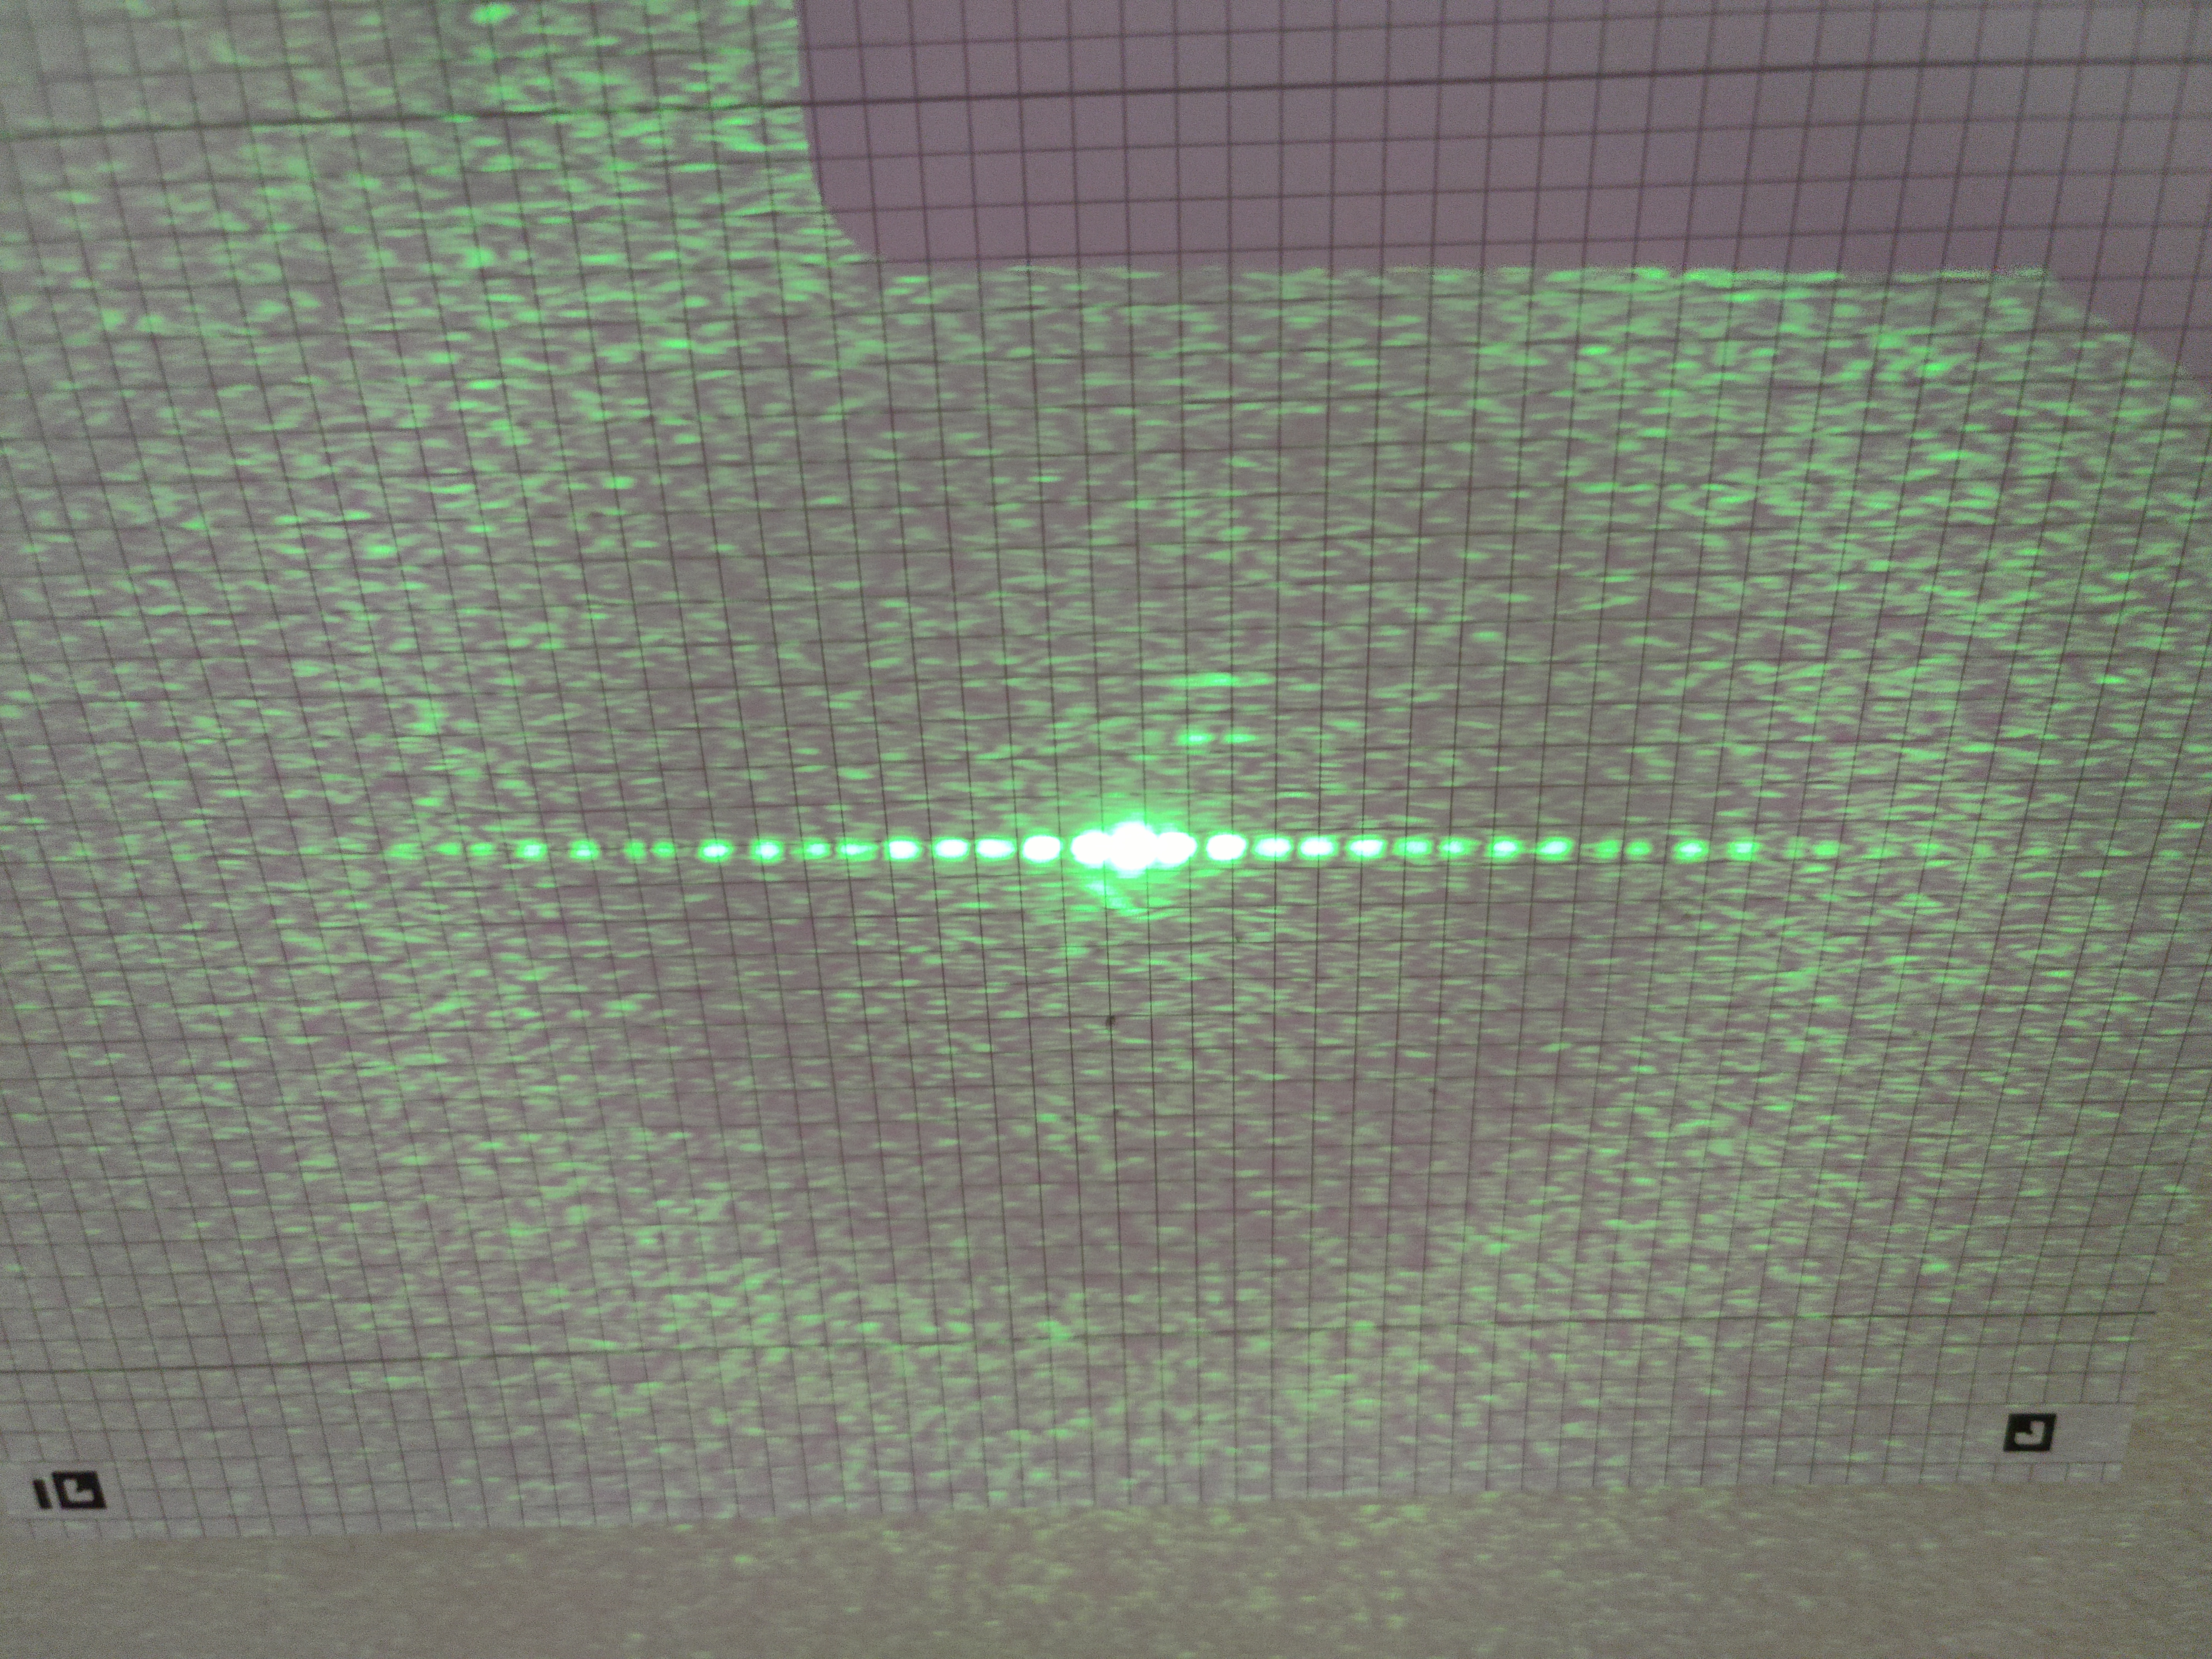
\includegraphics[width=\linewidth]{fig/DS1_0_20_25.jpg}
        \caption{Interferenzmuster des Doppelspalts $i = 1$}
        \label{fig:DS_1_interferenzmuster}
        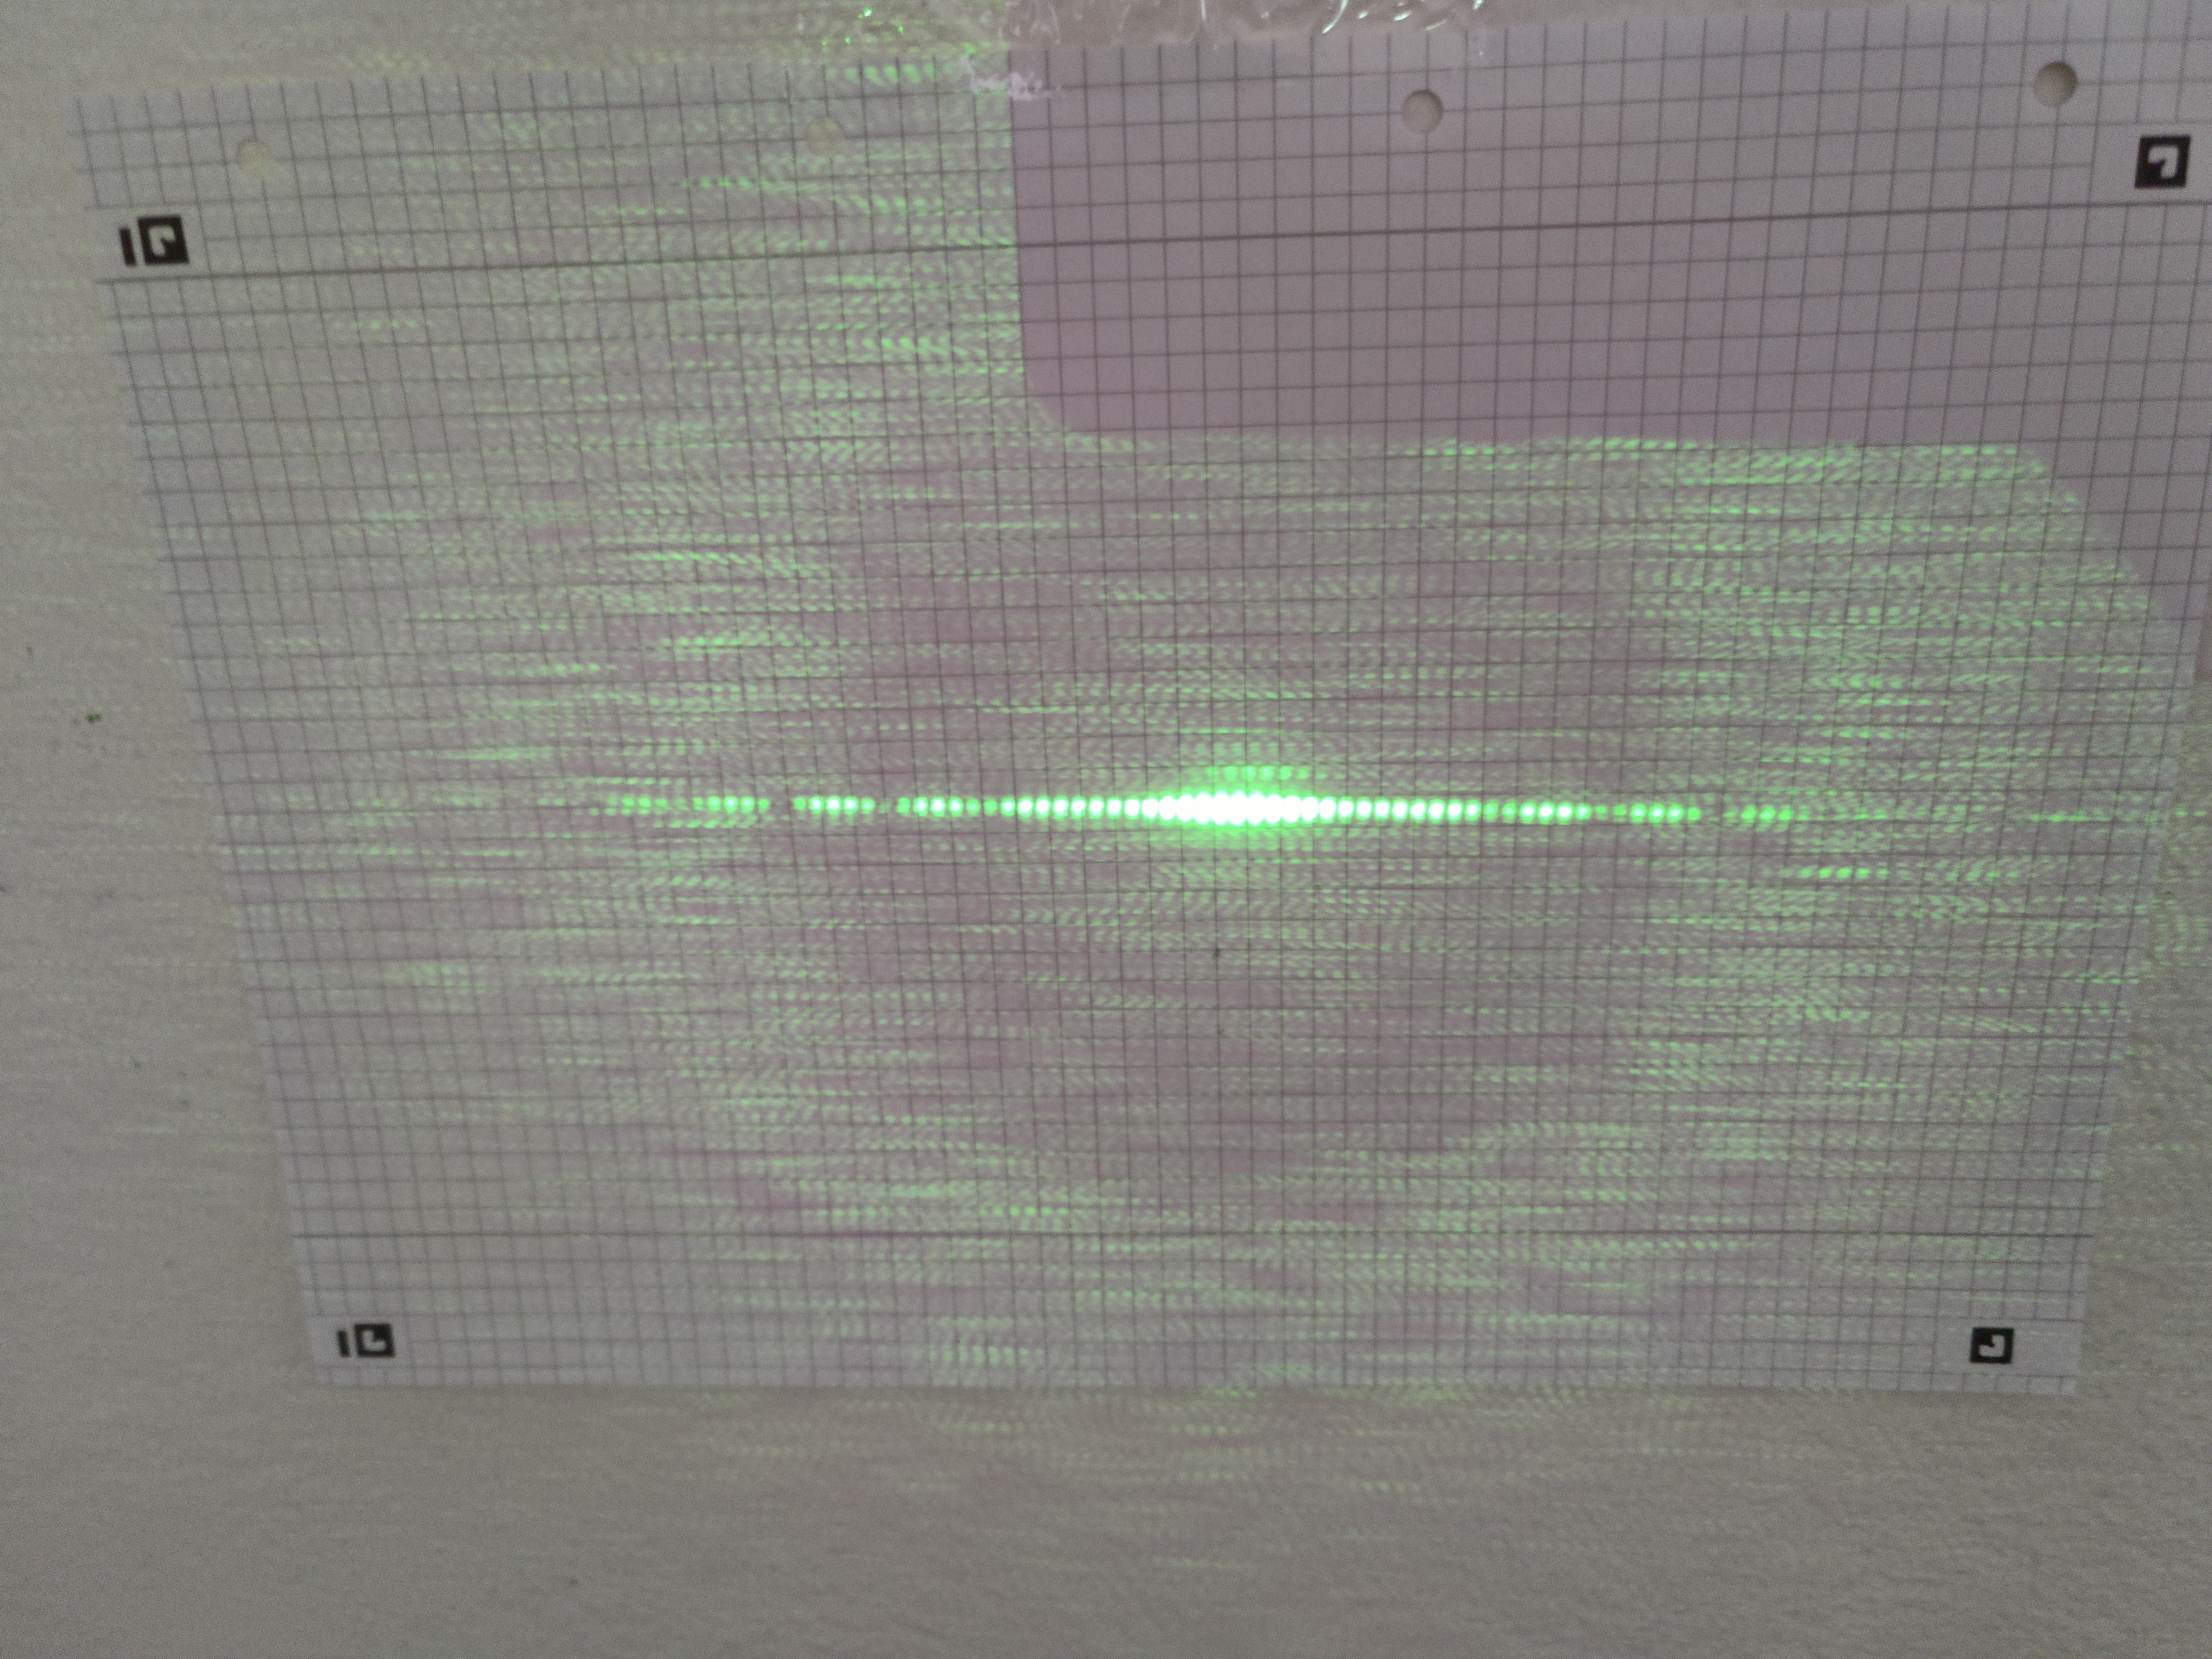
\includegraphics[width=\linewidth]{fig/DS3_0_10_5.jpg}
        \caption{Interferenzmuster des Doppelspalts $i = 3$}
        \label{fig:DS_3_interferenzmuster}
    \end{minipage}%
    \hspace*{\fill}
    \begin{minipage}[t]{0.45\linewidth}
        \centering
        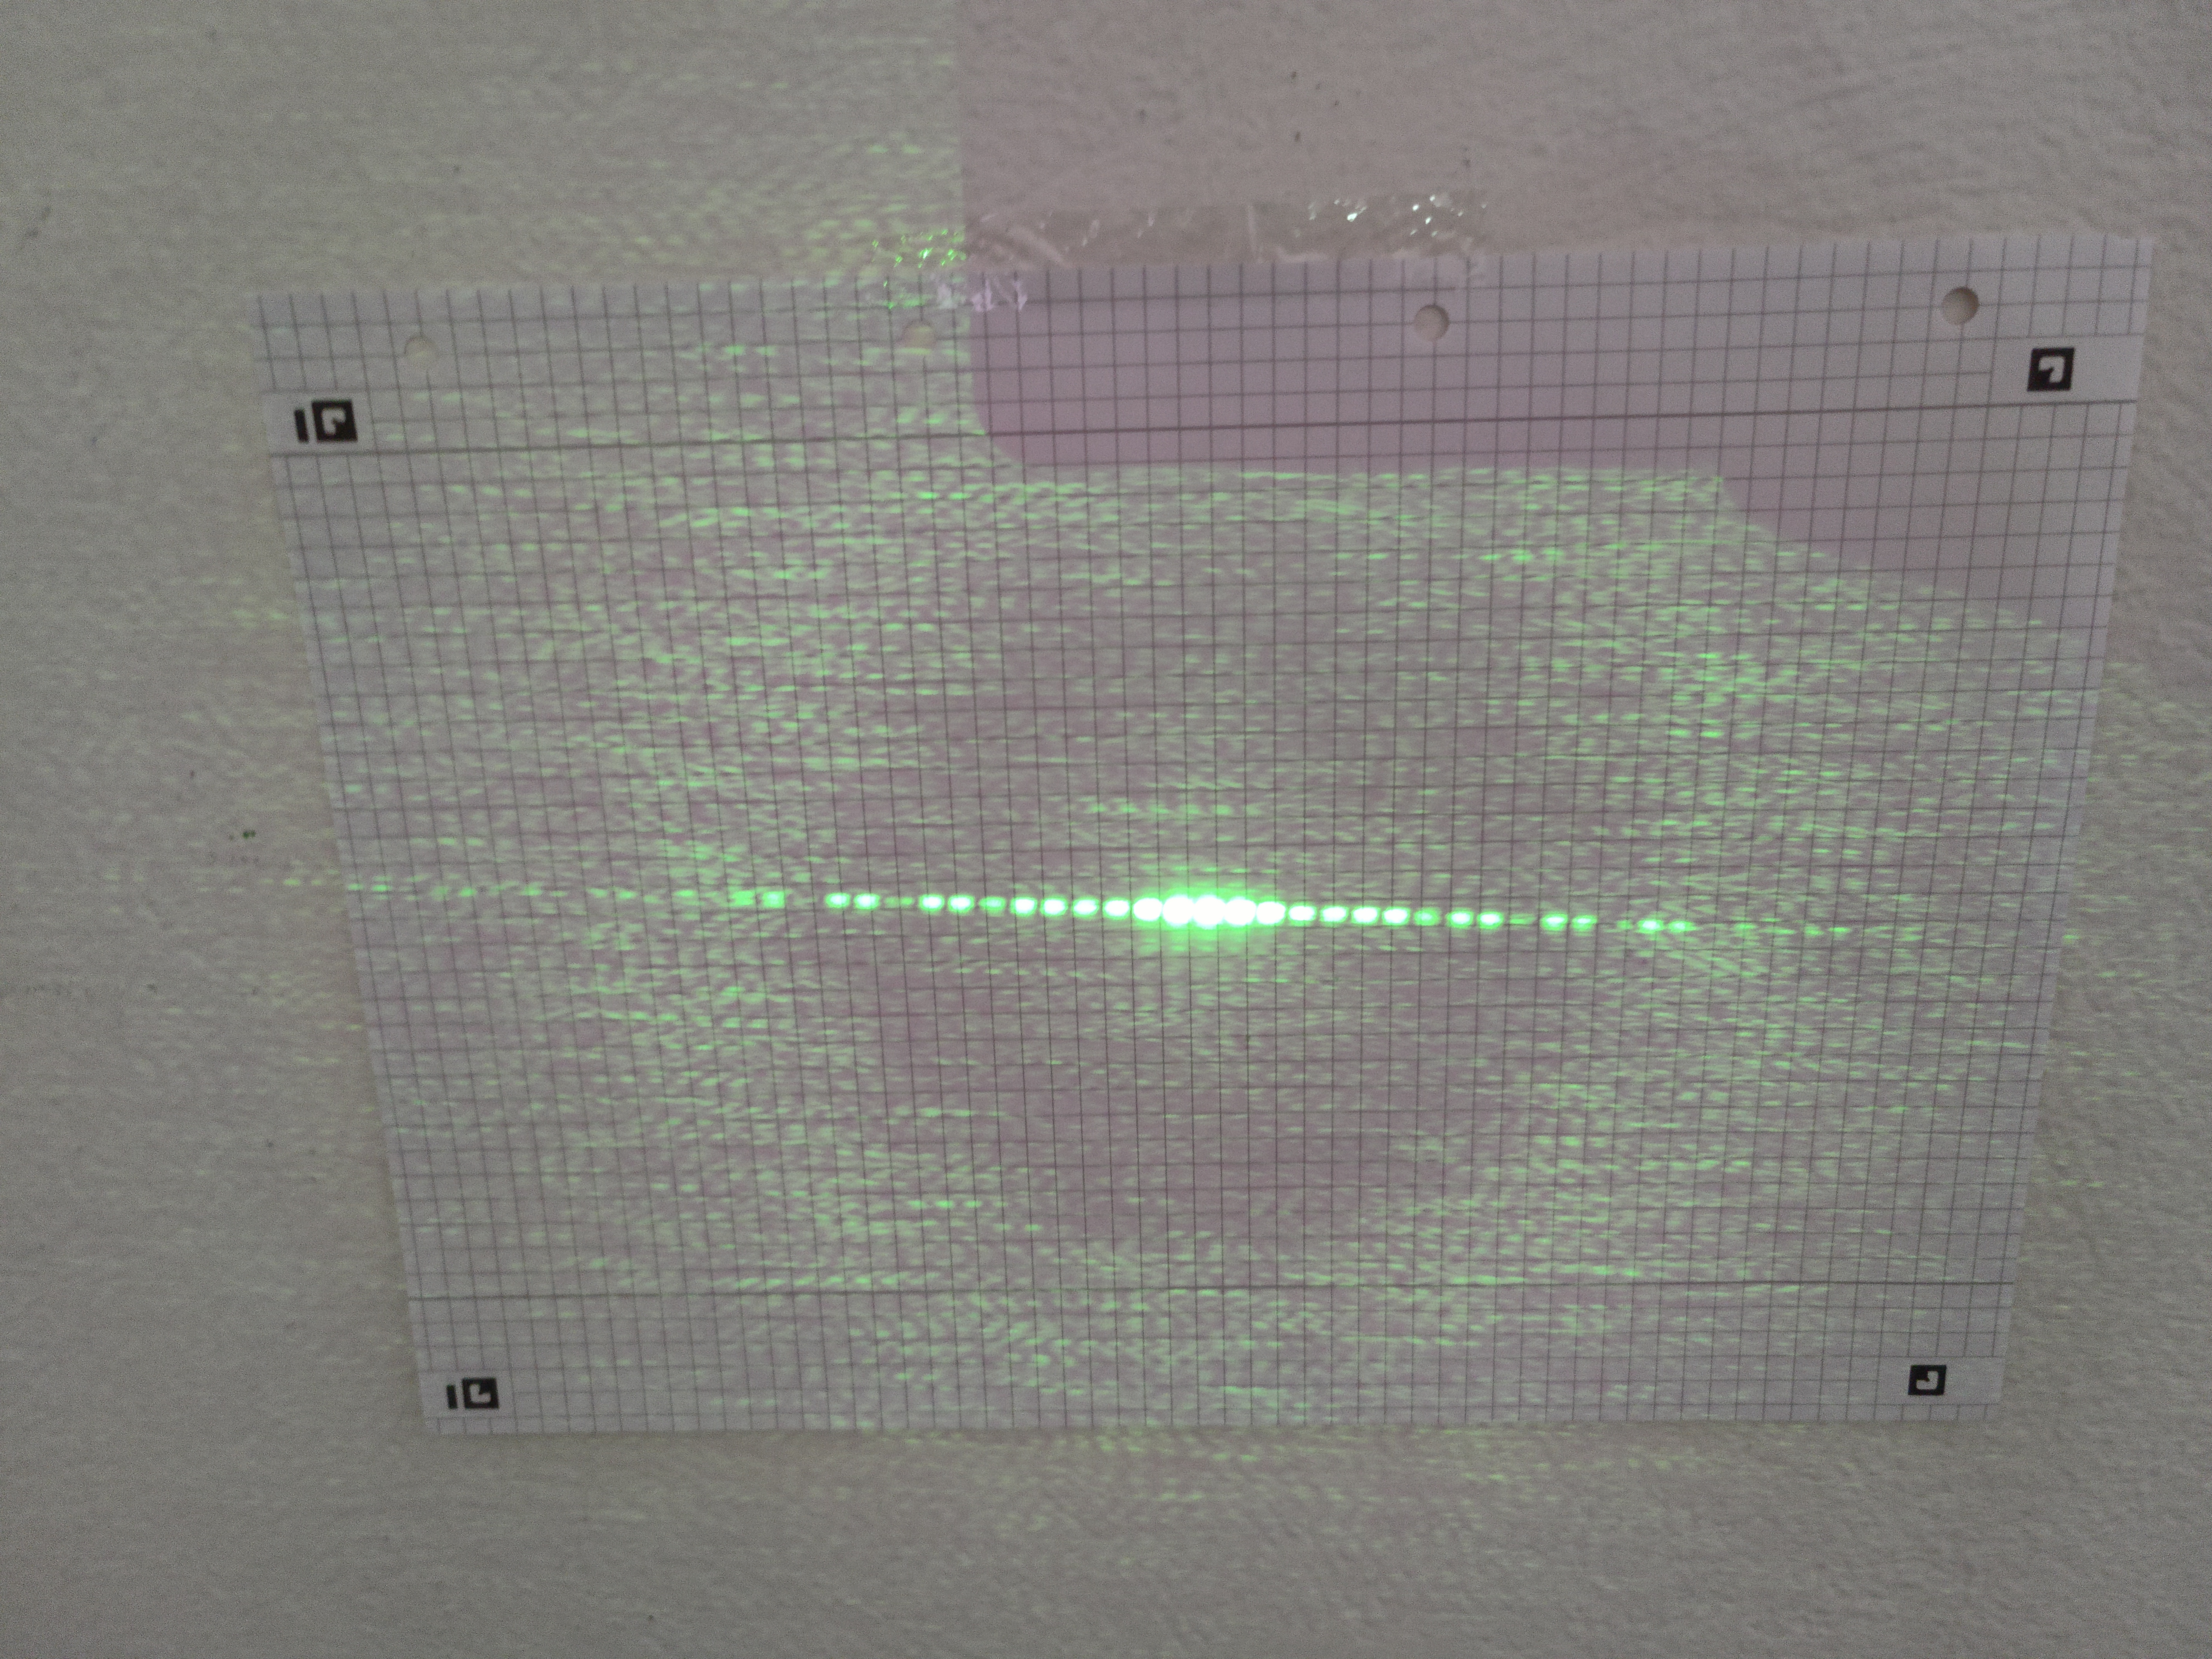
\includegraphics[width=\linewidth]{fig/DS2_0_10_25.jpg}
        \caption{Interferenzmuster des Doppelspalts $i = 2$}
        \label{fig:DS_2_interferenzmuster}
        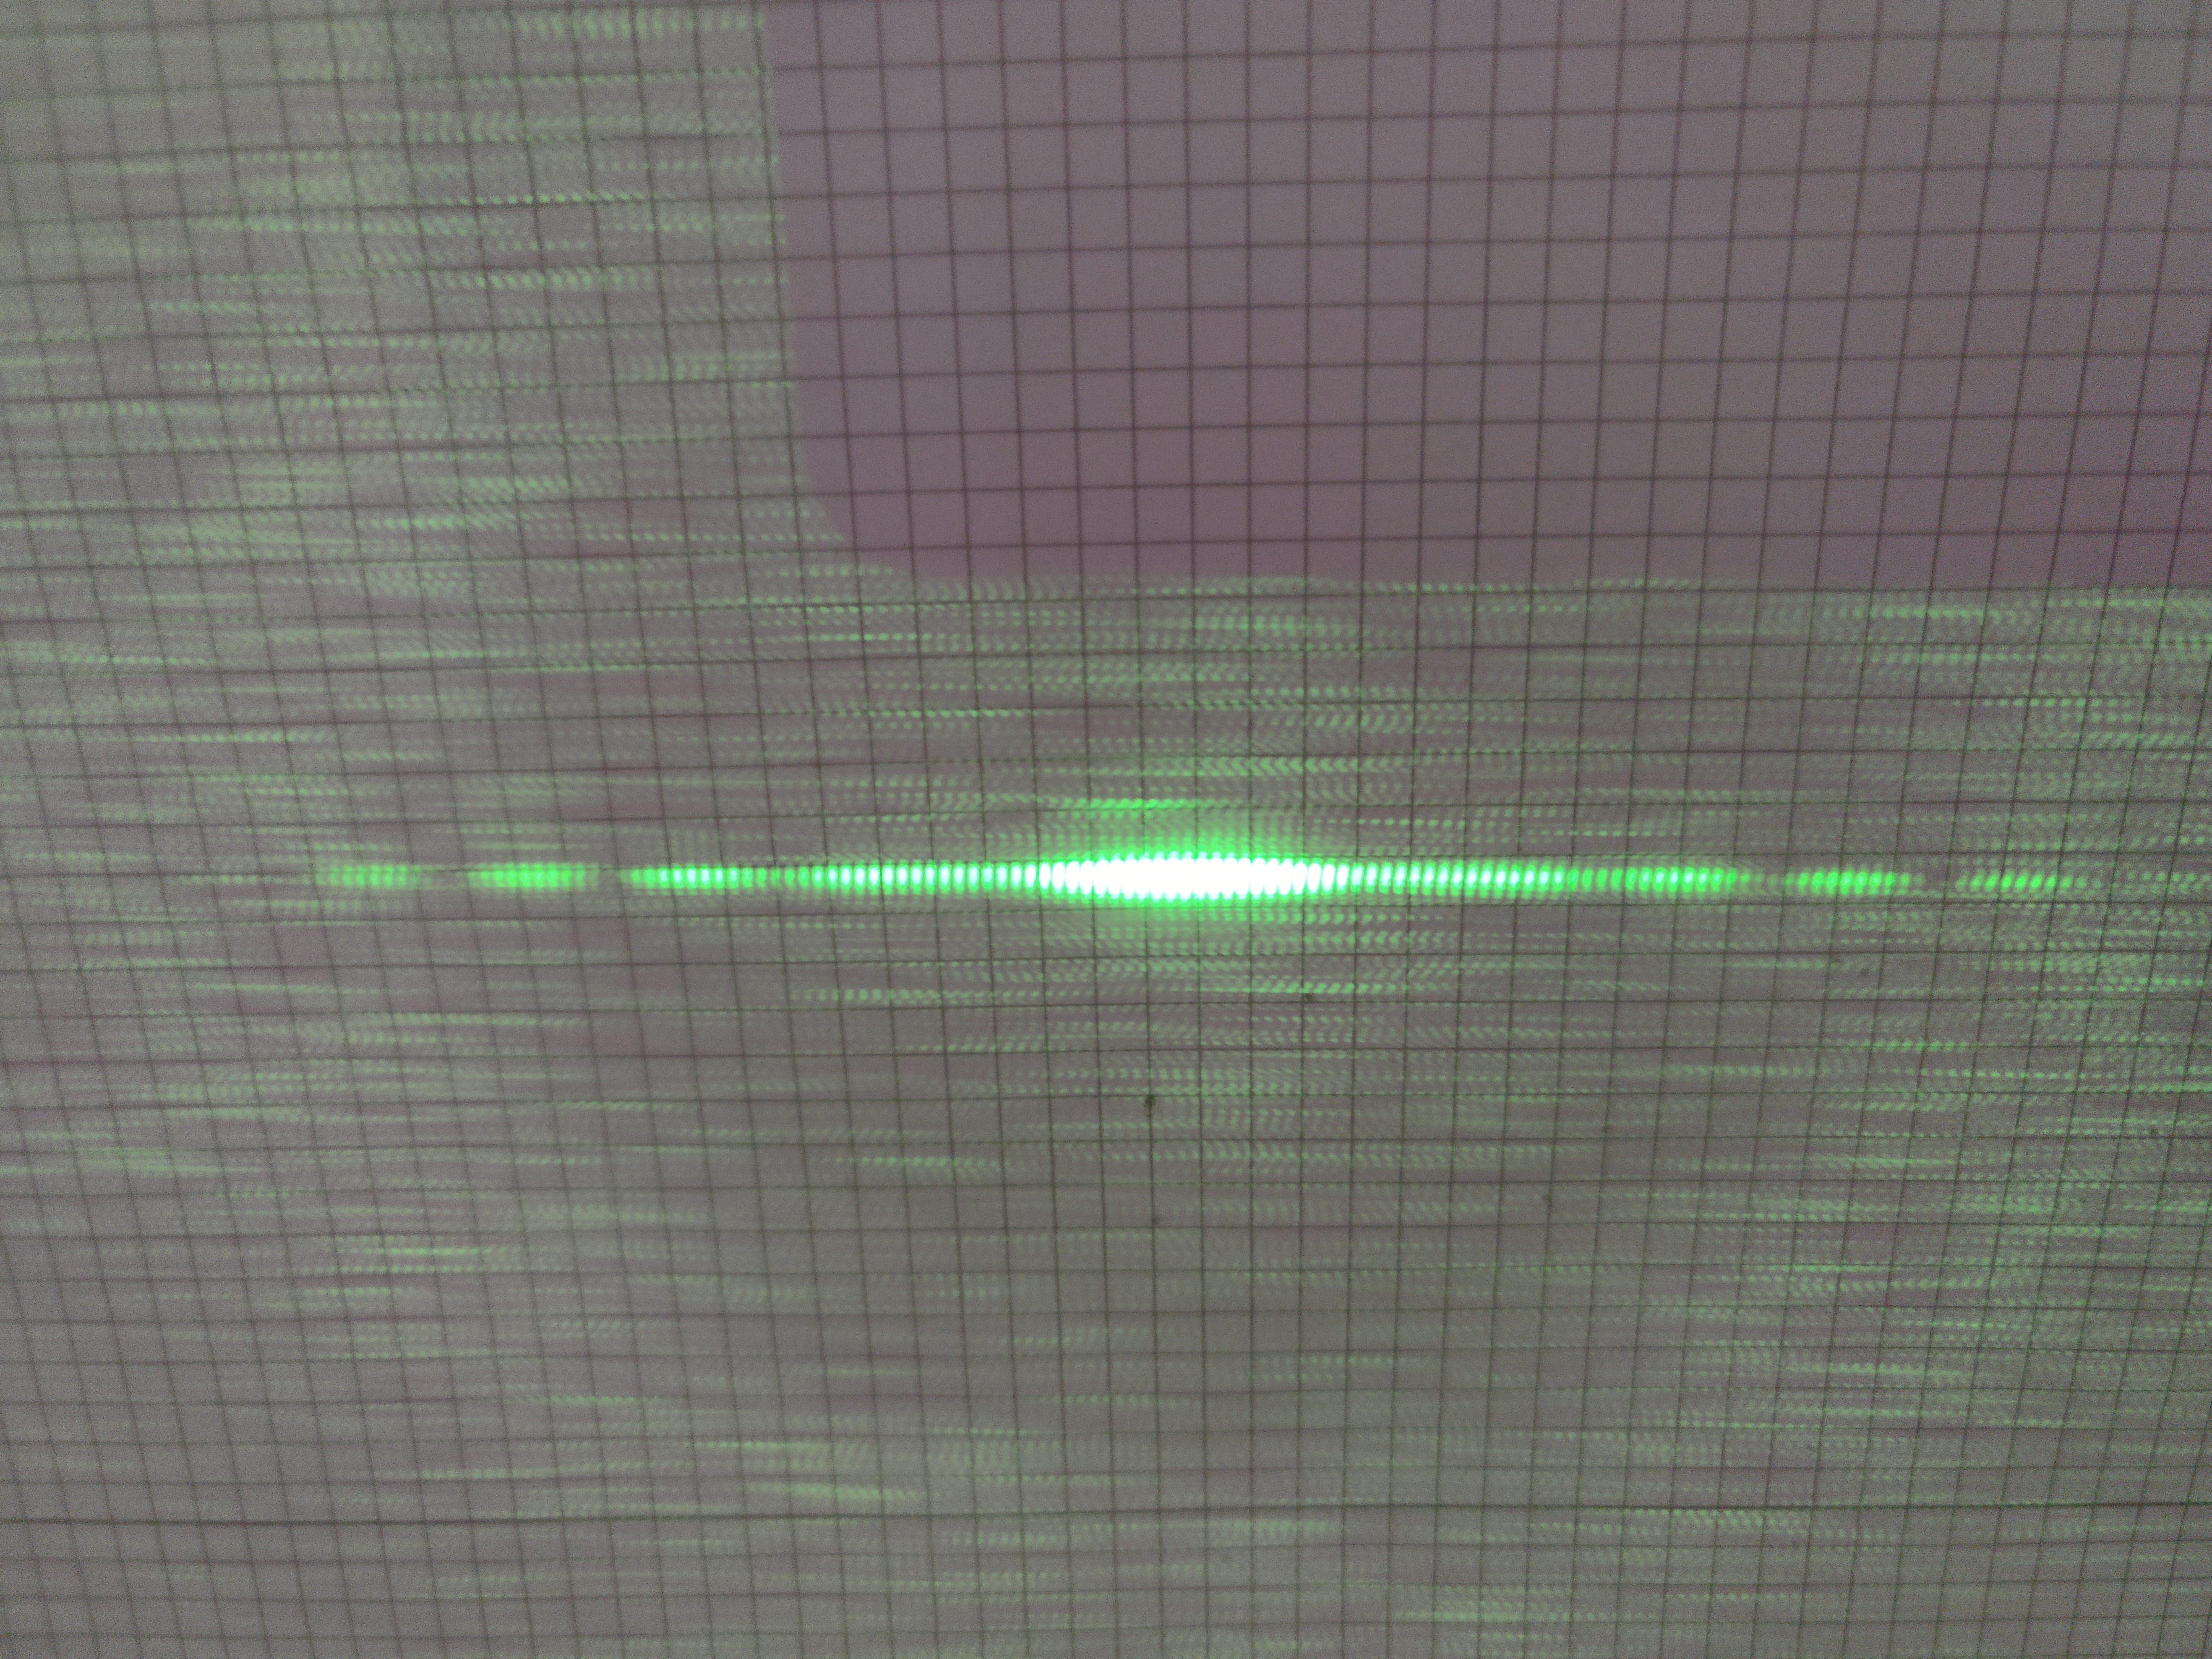
\includegraphics[width=\linewidth]{fig/DS4_0_11.jpg}
        \caption{Interferenzmuster des Doppelspalts $i = 4$}
        \label{fig:DS_4_interferenzmuster}
    \end{minipage}
\end{figure}
\setcaphanging
%
Neben der fotografischen Dokumentation werden auch die Abstände der Maxima mittels Lineal vermessen. Die Messungen ergeben die in \autoref{tab:messwerte_doppelspalten} angeführten Werte.

%? Auf meinem laptop geht glaub i tabularray ned gescheit aber vermultich is es nur ein user error :D
\begin{table}[H]
    \centering
    \begin{samepage}
        \caption[Messwerte Doppelspalten]{Messwerte der Doppelspalten. Unsicherheit der Messung: $\Delta l_i = \SI{0.5}{\milli\meter}$}
        \label{tab:messwerte_doppelspalten}
        \begin{tblr}{colspec={cS[table-format=2.1] S[table-format=2.1] S[table-format=2.1] S[table-format=2.1]}, row{1}={guard}}
            $i$ & $l_1$ / \unit{\milli\meter} & $l_2$ / \unit{\milli\meter} & $l_3$ / \unit{\milli\meter} & $l_4$ / \unit{\milli\meter} \\
            0   & 0.0                         & 0.0                         & 0.0                         & 0.0                         \\
            1   & 5.0                         & 5.0                         & 2.5                         & 1.5                         \\
            2   & 11.0                        & 11.0                        & 8.0                         & 2.5                         \\
            3   & 16.0                        & 16.0                        & 10.5                        & 4.0                         \\
            4   & 21.0                        & 22.0                        & 13.0                        & 5.5                         \\
            5   & 27.0                        & 27.0                        & 16.0                        & 6.5                         \\
            6   & 33.0                        & 32.0                        & 18.5                        & 8.0                         \\
            7   & 38.0                        & 38.0                        & 21.0                        & 9.5                         \\
            8   & 43.0                        & 43.0                        & 24.0                        & 10.5                        \\
            9   & 49.0                        & 48.0                        & 26.5                        & 12.0                        \\
            10  & 55.0                        & 54.0                        & 29.0                        & 13.5                        \\
            11  & 58.0                        & {{{-}}}                     & {{{-}}}                     & 15.0                        \\
        \end{tblr}
    \end{samepage}
\end{table}

Die eben beschriebene Messung wird nun in analoger Weise nochmals mit dem Gitter durchgeführt. Die Messungen ergeben die in \autoref{tab:messwerte_gitter} angeführten Werte. Dabei bleibt der Abstand zum Schirm $l_\text{Schirm} = \SI{2520(5)}{\milli\meter}$ konstant.

\begin{table}[H]
    \centering
    \begin{samepage}
        \caption[Messwerte Gitter]{Messwerte des Gitters. Unsicherheit der Messung: $\Delta l_i = \SI{0.5}{\milli\meter}$}
        \label{tab:messwerte_gitter}
        \begin{tblr}{colspec={c S[table-format=3.1]}, row{1}={guard}}
            $i$ / 1 & $l_1$ / \unit{\milli\meter} \\
            0       & 0.0                         \\
            1       & 11.0                        \\
            2       & 21.5                        \\
            3       & 32.5                        \\
            4       & 43.0                        \\
            5       & 53.5                        \\
            6       & 64.5                        \\
            7       & 75.0                        \\
            8       & 86.0                        \\
            9       & 97.0                        \\
            10      & 108.0                       \\
            11      & 118.0                       \\
            12      & 128.0                       \\
            13      & 139.0                       \\
            14      & 151.0                       \\
        \end{tblr}
    \end{samepage}
\end{table}


\subsection{Shearing-Interferometer}
\label{sec:durchfuehrung_shearing}

Nachdem der Versuchaufbau ordnungsgemäß hergestellt ist, wird der Laser eingeschaltet. Am optischen Ausgang am oberen Ende des Shearing-Interferometers erscheint dadurch ein streifenförmiges Interferenzmuster. Aus diesem Interfenzmuster werden der Versatz in laterale Richtung $l$, der Abstand der Interferenzstreifen $d$ und der Winkelversatz zur einfallenden Ebene $\theta$ vermessen. Vermessen wurde direkt am optischen Ausgang mit einem handelsüblichen durchsichtigen Geodreieck. Für die Längenmessung wird eine Ableseunsicherheit von \SI{0.5}{mm} angenommen, die Winkelmessung wird mit einer Ungenauigkeit von \SI{3}{\degree} abgeschätzt. Aufgrund der hohen Messungenauigkeit dieser Methodik wird die Messung zwei weitere Male wiederholt, um so zumindest eine geringfügige statistische Aussage treffen zu können. Die Messergebnisse werden notiert und tabelliert.
\begin{table}[H]
    \centering
    \begin{samepage}
        \caption[Messung Shearing]{Gemessene Größen beim Versuchsaufbau Shearing-Interferometer mit $l$ Versatz in laterale Richtung, $d$ dem Abstand der Interferenzstreifen $\theta$ und dem Winkelversatz zur einfallenden Ebene. }
        \label{tab:}
        \begin{tblr}{colspec={}, row{1}={guard}}
        \end{tblr}
    \end{samepage}
\end{table}

%!Natürlich komplett frei erfunden
\begin{itemize}
    \item $l$ = \SI{8.0(5)}{\milli\meter}
    \item $\Theta$ = \SI{-19(3)}{\degree}
    \item $d$ = \SI{4.0(5)}{\milli\meter}
\end{itemize}





\subsection{Polarisation}
\label{sec:durchfuehrung_polarisation}
Der Strahl wird für den ersten Unterpunkt dieses Versuchs durch zwei Polarisationsfilter geführt. Für den ersten der beiden Filter wurde \SI{70}{\degree} als Ausgangswinkel gewählt, der zweite wird im folgenden Versuch einmal um \SI{360}{\degree} gedreht, wobei die Ausgangsstellung hier so gewählt wird, dass zuerst die höchste Lichtintensität am Messgerät abgelesen werden kann. So stehen die Polarisationsfilter gleich; Dies ist bei \SI{330}{\degree} des zweiten Filters der Fall.
Die Messung wurde zweimal durchgeführt und die gemessenen Werte des Lichtintensitätsmesser sind in \autoref{tab:messwerte_polarisation} angeführt.
% \begin{table}[H] 
%     \centering
%     \begin{samepage}
%         \caption[Messwerte Polarisation]{Messwerte nach Durchgang durch zwei Polarisationsfilter \\Winkel des ersten Filters: \SI{70}{\degree}, Winkel des zweiten Filters $\alpha$ mit $\Delta \alpha$ = \SI{3}{\degree}, Intensität $I$ }
%         \label{tab:messwerte_polarisation}
%         \begin{tblr}{colspec={S[table-format=3.0]S[table-format=4.0]S[table-format=4.0]}}
%             {{{$\alpha$}}} & {{{$I_1$ / \unit{\lux}}}}& {{{$I_2$ / \unit{\lux}}}} & {{{$\Delta I_1$ / \unit{\lux}}}} & {{{$\Delta I_2$ / \unit{\lux}}}} \\
% 330.0   & 1022.0        & 1074.0        & 40.66         & 42.22 \\
% 340.0   & 999.0         & 1050.0        & 39.97         & 41.5  \\
% 350.0   & 911.0         & 966.0         & 37.33         & 38.98 \\
% 0.0     & 781.0         & 820.0         & 33.43         & 34.6  \\
% 10.0    & 617.0         & 643.0         & 28.51         & 29.29 \\
% 20.0    & 444.0         & 456.0         & 23.32         & 23.68 \\
% 30.0    & 279.0         & 285.0         & 18.37         & 18.55 \\
% 40.0    & 132.0         & 142.0         & 13.96         & 14.26 \\
% 50.0    & 37.0  & 38.0  & 11.11         & 11.14 \\
% 60.0    & 0.0   & 0.0   & 10.0  & 10.0  \\
% 70.0    & 24.0  & 26.0  & 10.72         & 10.78 \\
% 80.0    & 108.0         & 110.0         & 13.24         & 13.3  \\
% 90.0    & 236.0         & 252.0         & 17.08         & 17.56 \\
% 100.0   & 397.0         & 412.0         & 21.91         & 22.36 \\
% 110.0   & 578.0         & 603.0         & 27.34         & 28.09 \\
% 120.0   & 756.0         & 793.0         & 32.68         & 33.79 \\
% 130.0   & 896.0         & 943.0         & 36.88         & 38.29 \\
% 140.0   & 1000.0        & 1046.0        & 40.0  & 41.38 \\
% 150.0   & 1047.0        & 1097.0        & 41.41         & 42.91 \\
% 160.0   & 1028.0        & 1074.0        & 40.84         & 42.22 \\
% 170.0   & 950.0         & 993.0         & 38.5  & 39.79 \\
% 180.0   & 816.0         & 847.0         & 34.48         & 35.41 \\
% 190.0   & 653.0         & 679.0         & 29.59         & 30.37 \\
% 200.0   & 471.0         & 490.0         & 24.13         & 24.7  \\
% 210.0   & 288.0         & 304.0         & 18.64         & 19.12 \\
% 220.0   & 150.0         & 150.0         & 14.5  & 14.5  \\
% 230.0   & 38.0  & 43.0  & 11.14         & 11.29 \\
% 240.0   & 0.0   & 0.0   & 10.0  & 10.0  \\
% 250.0   & 25.0  & 24.0  & 10.75         & 10.72 \\
% 260.0   & 114.0         & 121.0         & 13.42         & 13.63 \\
% 270.0   & 257.0         & 263.0         & 17.71         & 17.89 \\
% 280.0   & 421.0         & 440.0         & 22.63         & 23.2  \\
% 290.0   & 607.0         & 635.0         & 28.21         & 29.05 \\
% 300.0   & 747.0         & 819.0         & 32.41         & 34.57 \\
% 310.0   & 927.0         & 971.0         & 37.81         & 39.13 \\
% 320.0   & 1029.0        & 1070.0        & 40.87         & 42.1  \\
% 330.0   & 1067.0        & 1109.0        & 42.01         & 43.27 \\
%         \end{tblr}
%     \end{samepage}
% \end{table}


\subsection{Michelson Interferometer}
\label{sec:durchfuehrung_michelson}



\section{Auswertung}
\label{sec:auswertung}

% \setcapindent{0pt}
% \begin{figure}[H]
%     \centering
%     \begin{minipage}[t]{0.45\linewidth}
%         \centering
%         \includegraphics[width=\linewidth]{plots/stern_allgemein.png}
%         \caption[Zeigerdiagramm allgemeine Sternschaltung]{Zeigerdiagramm allgemeine Sternschaltung, Strom $I_{xx}$ in \si{\centi\ampere} und Spannung $U_{xx}$ in \si{\volt}}
%         \label{fig:stern_asym_allg_zeigerdiagramm}
%     \end{minipage}%
%     \hspace*{\fill}
%     \begin{minipage}[t]{0.45\linewidth}
%         \centering
%         \includegraphics[width=\linewidth]{plots/stern_allgemein_tausch.png}
%         \caption[Zeigerdiagramm allgemeine Sternschaltung mit vertauschten Außenleitern ($\text{L2} \leftrightarrow \text{L3}$)]{Zeigerdiagramm allgemeine Sternschaltung mit vertauschten Außenleitern ($\text{L2} \leftrightarrow \text{L3}$), Strom $I_{xx}$ in \si{\centi\ampere} und Spannung $U_{xx}$ in \si{\volt}}
%         \label{fig:stern_asym_allg_tausch_zeigerdiagramm}
%     \end{minipage}
% \end{figure}
% \setcaphanging




\section{Diskussion}
\label{sec:diskussion}


\section{Zusammenfassung}
\label{sec:zusammenfassung}


\clearpage
% Literaturverzeichnis
\printbibliography

% Abbildungsverzeichnis
\listoffigures

% Tabellenverzeichnis
\listoftables


\end{document}